\documentclass[12pt,a4paper,twoside]{book}

%%%%%%%%%%%%%%%%%%%%%%%%%%%%%%%%%%%%%%%%%%%%%%%%%%%%%%%%%%%%%%%%%%%%%%%%
%%%%%%%%%%%% Packages %%%%%%%%%%%%%%%%%%%%%%%%%%%%%%%%%%%%%%%%%%%%%%%%%%
%%%%%%%%%%%%%%%%%%%%%%%%%%%%%%%%%%%%%%%%%%%%%%%%%%%%%%%%%%%%%%%%%%%%%%%%

%%%%%%
% In general useful packages
%%%%%%
%\usepackage[square,sort,comma,numbers]{natbib}
\usepackage{multirow}
\usepackage{longtable}
\usepackage[square]{natbib}
\usepackage[latin1]{inputenc} % allow Umlauts
\usepackage[T1]{fontenc} % Umlauts as character in font
\usepackage{fancyhdr}   % Header/Footer
\usepackage[pdftex]{graphicx}
\usepackage{pdfpages}
\usepackage{float}
\usepackage{fancyvrb}   % extended verbatim environment
\usepackage{amsmath}
\usepackage{algorithm}
\usepackage[noend]{algpseudocode}
\usepackage[most]{tcolorbox}
\usepackage{subfig}
\usepackage{stmaryrd}
%\raggedbottom
\makeatletter
\def\BState{\State\hskip-\ALG@thistlm}
\makeatother
\usepackage[us]{datetime} % date in \today as "Month DD, YYYY", e.g., "February 29, 2012"
\usepackage[plainpages=false, pdfpagelabels, bookmarks,  colorlinks=false,
linkbordercolor={0 0 1}, filebordercolor={0 0 1}, citebordercolor={0 0 1},
menubordercolor={0 0 1}, urlbordercolor={0 0 1}]{hyperref}

\usepackage{pdfcomment}  % comments in text as PDF notes
\newenvironment{nscenter}
{\parskip=0pt\par\nopagebreak\centering}
{\par\noindent\ignorespacesafterend}

%%%%%%%%%%%%%%%%%%%%%%%%%%%%%%%%%%%%%%%%%%%%%%%%%%%%%%%%%%%%%%%%%%%%%%%%
%%%%%%%%%%%% Layout %%%%%%%%%%%%%%%%%%%%%%%%%%%%%%%%%%%%%%%%%%%%%%%%%%
%%%%%%%%%%%%%%%%%%%%%%%%%%%%%%%%%%%%%%%%%%%%%%%%%%%%%%%%%%%%%%%%%%%%%%%%
% German style (no paragraph indent, but gap between paragraphs)
% \setlength{\parindent}{0mm}
% \setlength{\parskip}{4pt plus3pt minus2pt}

% Page width and margins (usually no need to change, just use a4wide package)
% \setlength{\textwidth}{15cm}
% \addtolength{\oddsidemargin}{1mm}
% \addtolength{\evensidemargin}{-13.5mm}
\usepackage{a4wide} % better than individual setup

% For fancyhdr, otherwise it might result in "overfull vbox"
\addtolength{\headheight}{3.5pt}

% URL Prefix for Bibliography (i.e., no prefix, typewriter as font for URLs)
\newcommand{\urlprefix}{}
\def\UrlFont{\small\tt}
%\urlstyle{rm} % oder sf, falls obiges nicht funktioniert


%%%%%%%%%%%%%%%%%%%%%%%%%%%%%%%%%%%%%%%%%%%%%%%%%%%%%%%%%%%%%%%%%%%%%%%%
%%%%%%%%%%%% Some useful macros %%%%%%%%%%%%%%%%%%%%%%%%%%%%%%%%%%%%%%%%
%%%%%%%%%%%%%%%%%%%%%%%%%%%%%%%%%%%%%%%%%%%%%%%%%%%%%%%%%%%%%%%%%%%%%%%%

% myfigure: filename width caption
\newcommand{\myfigure}[3]{%
	\begin{figure}
		\centerline{\includegraphics[width=#2]{figures/#1.pdf}}
		\caption{#3}
		\label{fig:#1}
	\end{figure}
}

% Floating figures = figures with floating text around: filename width caption
\newcommand{\myfloatfigure}[3]{%
	\begin{floatingfigure}{#2}
		\includegraphics[width=#2]{figures/#1.pdf}
		\caption{#3}
		\label{fig:#1}
	\end{floatingfigure}
}

% two figures side by side: file1 width1 caption1 file2 width2 caption2
\newcommand{\mydoublefigure}[6]{%
	\begin{figure}
		\begin{minipage}[t]{#2}
			\centerline{\includegraphics[width=\textwidth]{figures/#1.pdf}}
			\centering
			\caption{#3}
			\label{fig:#1}
		\end{minipage}
		\hfill
		\begin{minipage}[t]{#5}
			\centerline{\includegraphics[width=\textwidth]{figures/#4.pdf}}
			\centering
			\caption{#6}
			\label{fig:#4}
		\end{minipage}
	\end{figure}
}


% Better verbatim environments (requires fancyvrb package)
\DefineVerbatimEnvironment{myverb}{Verbatim}{fontsize=\small,baselinestretch=0.84}
\DefineVerbatimEnvironment{myverbbox}{Verbatim}{frame=single,fontsize=\small,baselinestretch=0.84}


% For figures and tables
\renewcommand{\topfraction}{0.9} % a page has at most 90% of floats and at least 10% of text (if page contains floats AND text)
\renewcommand{\bottomfraction}{0.9}
\renewcommand{\floatpagefraction}{0.7} % a page with floats only is at least 70% full

% Hyphenation (include a special file with hyphenation hints if there are problems)
% \include{myhyphen}

\begin{document}
	
	\raggedbottom
	% Title page
	
	\begingroup
	\pagenumbering{roman}
	%\thispagestyle{empty}
%\setcounter{page}{1}

\vspace*{3cm}
\centerline{{\Large\bf Improving Word Embeddings\\ Using Kernel Principal Component Analysis}}
\vspace*{4mm}

\centerline{{\Large\bf}}

\vspace{2cm}


\centerline{Master Thesis }
% include the title of your programme
\centerline{Media Informatics}

\vspace{2cm}

\centerline{{\large Vishwani Gupta}}
\centerline{Matriculation number 351279}

\vspace{10mm}

% Date!
\centerline{\today}

\vspace{10mm}

\begin{center}
\begin{minipage}[t]{8cm}
Supervisors: \\
\hspace*{2cm} Prof. Dr. Christian Bauckhage \\
\hspace*{2cm} Prof. Dr. Stefan Wrobel\\[1cm]

\end{minipage}
\end{center}

	\begin{titlepage}
		\centering
		\vspace{1.5cm}
		{\huge Improving Word Embeddings Using Kernel Principal Component Analysis\bfseries \par}
		\vspace{2cm}
		{\Large\bfseries Vishwani Gupta\par}
		\vspace{2cm}
		{\bfseries Bonn-Aachen International Center for Information Technology (B-IT)\par}
		\vspace{3cm}
		{\Large Master Thesis\par}
		{\Large Media Informatics\par}
		\vspace{1cm}
		%{\Large Rheinische Friedrich-Wilhelms-Universit\"at Bonn \par}
		%{\Large Fraunhofer IAIS \par}
		
		\vspace{1cm}
		\vfill
		Supervisors\par
		Prof.~Dr.~Christian Bauckhage\par
		Prof.~Dr.~Stephan Wrobel
		
		\vfill
		
		% Bottom of the page
		%{\large \today\par}
		
	\end{titlepage}
	%\maketitle
	\newpage
	
	\thispagestyle{empty}
	
	\rule{0cm}{5cm}
	
	%%% Include abstract and acknowledgements as necessary
	\thispagestyle{empty}

\centerline{\Large{\textbf{Acknowledgements}}}

\vspace{2cm}

\noindent 
First and foremost, I would like to express my sincere gratitude to Prof.~Dr.~Christian Bauckhage for his continuous support during this thesis. He has not only been my supervisor but also a very inspirational figure during my Master's studies. This is my heartfelt thanks for his motivational lectures which have helped me to improve as a computer science student and pursue the field of machine learning. \\\\
I would also like to offer my gratitude to Prof.~Dr.~Stephan Wrobel for supervising this thesis. His work in the field of machine learning has always been an inspiration for me.\\\\
To my life coach, my grandfather, and my father, I would like to dedicate all that I have achieved till date because they are the reason for what I am today. I look up to them as they never stop giving their hundred percent even when things get difficult and inspire me to do the same. I would also acknowledge my mom and my siblings for always having my back. I would also like to acknowledge my gratitude to Mr. Ankit Gupta, co-founder Pulse, who not only has motivated me to challenge myself daily but also has inspired me to do my best.\\\\
I also extend my gratitude towards Mr.Sven Giesselbach and Dr.Tim Wirtz for being very understanding and supporting during my thesis completion. Last but not least, I am grateful towards my friends who have always supported me during these months.


\newpage
\thispagestyle{empty}

\rule{0cm}{5cm}

	\thispagestyle{empty}

\centerline{\Large{\textbf{Abstract}}}

\vspace{2cm}
Word embeddings have always been an active and crucial research area in the field of Natural Language Processing. This is because of the fact that most of the NLP algorithms use word embeddings at their atomic level. Since this constitutes the backbone of most of the NLP algorithms, researchers, continuously explore ways to make the models which generate these embeddings, more efficient. Some popular models used for generating these embeddings includes distributive skip gram model and CBOW model. These models learn a distributed vector representations that capture a large number of precise syntactic and semantic word relationships. Both of these models, when learning the vector representation of the words, take only the context of the word into account. The sub-structure of the words, which plays a very important role in morphologically rich languages are not taken into account. A more recent model, known as fastText has used an approach to generate word embeddings based on n-grams of the words. This approach learns the vector representation of the word as well as the n-grams in the word, hence enriching the word embedding with sub word vectors.
In this thesis work, we have also tried to follow the approach of enriching the word embeddings, generated using the skip gram model, with the morphological information. This morphological information is derived from computing the KPCA of the words in the vocabulary. One benefit of using the KPCA embeddings of the vocabulary is that it can very easily be extended for the out-of-vocabulary words. Once we have the KPCA embeddings of the words, we can very easily use them as input vectors in the skip gram model. This can be seen as explicitly feeding the network with morphological similarities of the words and letting the network learn semantic and syntactic similarities. We can also see this approach as a better initialization of the model. When we evaluate our approach on the word similarity and analogy tasks, we found that our approach not only achieved better accuracies than the basic skip gram model but also fasten the process of training. We also explored the idea of training a skip gram model fed with KPCA embeddings, on a relatively smaller dataset. In contrast to the basic skip gram model, which needs to be trained on a large dataset to generate meaningful word embeddings, our model can be trained on a smaller dataset and yet produces good quality word embeddings. This approach not only works quite well for a morphologically rich language but also works fairly well for the non-morphological languages. 
\newpage
\thispagestyle{empty}
\rule{0cm}{5cm}
	
	\newpage
	\endgroup
	
	\pagestyle{fancy}
	
	% Headers with page numbers and section/chapter titles
	\renewcommand{\sectionmark}[1]{\markright{\thesection\ #1}}
	\renewcommand{\chaptermark}[1]{\markboth{\thechapter\ #1}{}}
	\lhead[\rm\thepage]{\sl\rightmark}
	\chead{}
	\rhead[\sl\leftmark]{\rm\thepage}
	
	% Footers empty\textbf{}
	\lfoot{}
	\cfoot{}
	\rfoot{}
	
	\tableofcontents
	\listoffigures
	\listoftables
	
	\newpage
	
	\chapter{Introduction}
\label{cha:intro}

% Important: you have to switch to arabic numbering here!
\pagenumbering{arabic}
\section{Motivation}
According to Prof. Andrew NG, artificial intelligence is like \textit{"the new electricity"}\footnote{https://www.gsb.stanford.edu/insights/andrew-ng-why-ai-new-electricity}. It has revolutionized every field in which it has found its use in. It has also enabled humans to be more efficient by managing their day to day tasks. Examples of such tasks include issuing commands to robots, comprehending the full text of newspaper articles or poetry passages, classifying text for the automatic analysis of emails and their routing to a suitable department. There have been many efforts invested to construct such an intelligent system.\\
A vital part of such a system is that it should easily understand human languages. \textit{"Natural language processing (NLP)"}, a field of AI, which deals with these problems. It can also be seen as a way through which computers can analyze, understand, and derive meaning from the human language. When computers understand our languages, they can organize and structure knowledge to perform tasks such as automatic summarization, translation, named entity recognition, relationship extraction, sentiment analysis, speech recognition, and topic segmentation etc. very efficiently.\\

\section{Challenges}
The NLP problems are not trivial, making them \textit{"AI-hard problem"} in the field of computer science. This can be attributed to the fact that human languages are not precise. In order to understand a sentence, one should not only understand the words used in it but also the context in which those words are used since a word can have very different meaning when used in different contexts. This makes language understanding ambiguous.\\
The solution comes by focusing on the "atomic units" of a language, \textbf{"words"}. To get the precise results, there is a dire need of a numeric vector representation for the words. These word representations help in extracting relations between various human languages, text or speech data. \\
One way to represent words is in their vectors representation. There are several advantages of using vector representations of the words which include application of the nearest neighbors algorithms on these vectors. When applied on the word, we can obtain clusters of similar meaning words. This can be very useful in text completion, next word prediction and in so many other applications.	

In order to build such a representation, a very basic idea was to use \texttt{one-hot vector}. One hot vector is a very sparse vector which has "1" at the index position of the word in the dictionary and "0" at all other positions. The main limitation of this vector representation is that it encodes no information about the word except its position in the given vocabulary. Such a vector representation depends on the vocabulary size of the text thus excluding the representations of \texttt{out-of-vocabulary words}.\\
To eliminate the first limitation, word embeddings which depends on the context of the text are being proposed. These embeddings are dense, low-dimensional and more informative than the one-hot vector encoding. To obtain such embeddings we need to train a neural network on a very huge amount of data. Such embeddings make use of semantic information of text such that words used in same context cluster together. What these models does not make use of, is the \texttt{sub-word information}. This does not effect so heavily when the language is non-morphological. But for the morphological languages like German and Turkish, we can do better as morphological similarity also embed semantic similarities between words and vice-versa. There have been some recent works such as \texttt{FastText}, which works on this idea of including sub-words in the vocabulary. The model is then trained on this increased vocabulary, learning vector representations of sub-words also. Although this approach eliminates both limitations of \texttt{one-hot vector}, there is significant increase in the vocabulary size which leads to the increased training time. This model still needs to be trained on a huge amount of data to generate high quality vectors.
\section{Thesis Outline}
In this work, we propose an alternative approach which not only make use of the sub-word information but also performs well on smaller datasets. This approach can be applied on both morphological and non-morphological languages. The main challenges we are trying to solve for generating word embeddings are:
\begin{enumerate}
	\item The need to train on a huge text corpus to extract relationship between words.
	\item Word embeddings for out-of-vocabulary words using \textit{n}-grams with significant increase in vocabulary size.
	\item Slow rate of training even after application of optimization techniques such as softmax and negative sampling.
\end{enumerate}
In Chapter 2, we provide all the theoretical background to understand the terminology and techniques used throughout this work. Following is the Chapter 3, which gives a quick overview of the related works dealing with generating word embeddings. Chapter 4 introduces and discusses the approach we proposed to meet the challenges mentioned above. Here we discuss in detail the steps from cleaning the data to obtaining kernel PCA embeddings and finally training a skip gram model for generating word embeddings using the KPCA embeddings. In Chapter 5, we compare our model, KPCA skip gram model with word2vec skip gram model trained using same parameters and finally conclude with Chapter 6 talking about the future work which involves further improvement in the proposed KPCA skip gram model and usage of embeddings in small datasets. 

	\chapter{Theory and Terminology}
\label{cha:solutioni}
In this chapter, we are going to discuss the theory and terminology used in this work.
Representing words in a vectorial form is an essential element in natural language processing. We have used a number of algorithms for getting such vector representations. In this chapter, we will briefly explain the background needed to understand those algorithms.
\section{Machine learning Algorithms at our disposal}

\subsection{Principle Component Analysis(PCA)}
Principal component analysis(PCA) is a very important tool in data analysis. It is a simple, non-parametric, mathematical tool that can be used in variety of fields where large amount of data is being generated. Importance of PCA can be understood from the fact that it can be very efficiently used in extracting information from a vague data set and is highly useful in dimensionality reduction. \\\\
In the real world settings, the data set which needs to be analyzed is generally very obscure and can be very high dimensional. This data usually have various outliers, errors or redundancy. Therefore preprocessing is vital before analyzing it. Even after preprocessing, it is difficult to figure out what this data is representing as it might be present in a high dimensional space. This makes it hard, not only to visualize but also to apply machine learning algorithms such as clustering or classification. Thus making "dimensionality reduction", very important in this data-driven world.\\ 
Data that is produced by various processes generally rely on a number of parameters but not all of these parameters are important for analyzing this data efficiently. An example of such a scenario is that if we have a naive experiment setting in which we do not know the underlying dynamics of the experiment. Then it is difficult to express this experiment as a function of some parameters.\\\\
"Principal Component Analysis(PCA)" helps in reducing a complex data set to a lower dimensional space thus revealing the hidden, dynamics. It helps in getting the most meaningful basis to re-express any noisy data set. The general consideration is that each data sample is represented in \textit{m}-dimensional space and all the vectors in such a space are in a linear combination of a set of unit basis vectors. PCA tries to explore some other basis, which best "re-expresses" the data and is a \textit{"linear"} combination of original basis. The main point to notice here is that PCA makes an assumption of \textbf{linearity}, thus making a limitation of re-expressing the data only as a linear combination of its basis vectors. Let $\mathbf{Y}$ is the re-expressed data set of the original data set, $\mathbf{X}$ and let $\mathbf{P}$ be the transformation matrix used in such a transformation. Then we can represent this basis transformation by the equation \ref{eq:pca}.
\begin{equation}\label{eq:pca}
\mathbf{PX = Y} 
\end{equation}
%\subsubsection{When to use PCA}
To understand how PCA finds the best solution for re-expressing $\mathbf{X}$ and for selecting a good choice for the basis transformation $\mathbf{P}$, one should understand what features, $\mathbf{Y}$ should have. When the data set is collected, it might contain: \textit{noise} and \textit{redundancy}.
\begin{enumerate}
	\item{Noise:} Noise should be as low as possible in a data set. A metrics to measure noise is \textit{Signal to noise ratio(SNR)} given by:
	\begin{equation}
	\mathit{SNR} = \dfrac{\sigma^2_{signal}}{\sigma^2_{noise}}
	\end{equation}
	where: $\sigma$ represents standard deviation and $\sigma^2$ represents the covariance.
	\item{Redundancy:} 
	Redundancy is also very important to deal with when it comes to dimensionality reduction. It is important to eliminate those dimensions which express the redundant information. This helps in eliminating dimensions which are not crucial without loosing information. 
\end{enumerate}
\subsubsection{Solving PCA with eigen value decomposition}
\subsubsection{Covariance Matrix}
Covariance matrix represents the strength of corelation between data points. If the data points are correlated in some way, then the covariance between these points will be nonzero and vice versa. While analyzing the covariance, the exact value is not as important as the sign of the values. If the value is positive, then this mean that the data points in question are increasing together. On the another hand, if the value is negative then this mean that when one increases, other one decreases. If the value is zero, then it means that both are independent of each other.\\
\begin{equation}
\sigma^2_A = \langle \mathit{a_ia_i} \rangle_i
\end{equation}
\begin{equation}
\sigma^2_B = \langle \mathit{b_ib_i} \rangle_i\\
\end{equation}
Covariance of $\mathit{A}$ and $\mathit{B}$ will be given by:
\begin{equation}
\sigma^2_{AB} = \langle \mathit{a_ib_i} \rangle_i
\end{equation}
\begin{equation}
\sigma^2_{AB} = \langle \mathit{(A-\mu_A)(B-\mu_B)} \rangle_i
\end{equation}
where: $\mu$ is the mean\\
The set of data points $\textbf{X}$, can be represented as row vectors matrix. In such a case, covariance, $\mathbf{S_X}$ can be calculated using:
\begin{center}
	$\mathbf{X} = [\mathbf{x}_1,\mathbf{x}_2 ... \mathbf{x}_n]^T$\\
\end{center}
\begin{center}
	$\mathbf{S_X} = \frac{1}{n-1}\mathbf{XX}^T$
\end{center}	
The main goal here is to minimize the redundancy, which is possible if the covariance between data points can be reduced. From interpretation of figure \ref{fig:redundancy}, to remove redundancy, the covariances between different data points should be zero. Let the "optimized covariance matrix" be $\mathbf{S_Y}$, then this matrix satisfies the above condition only when it is a diagonal matrix. 
\begin{figure}[H]
	\centering
	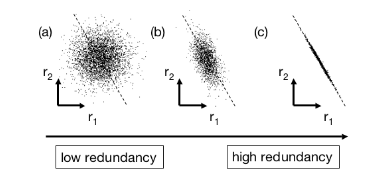
\includegraphics[width=10cm,height=12cm,keepaspectratio]{files/redundancy.png}
	\caption{A spectrum of possible redundancies in data for \textit{r1} and \textit{r2} (\cite{shlens2014tutorial})}
	\label{fig:redundancy}
\end{figure}
There are numerous ways to "diagonalize the covariance matrix" or to reduce noise and redundancy, but one of the easiest method is offered by PCA. The solution to PCA is based on \textit{eigenvectors} computation. 
The goal of PCA is to find an orthogonal matrix $\mathbf{P}$ where $\mathbf{Y = PX}$ such that $\mathbf{S_Y}$, in equation \ref{eq:diag}, is a diagonal matrix. \\
\begin{equation}\label{eq:diag}
\mathbf{S_Y = \frac{1}{(n-1)}YY^T}
\end{equation}
The rows of this orthogonal matrix, $\mathbf{P}$, are the principal components of $\mathbf{X}$. It can be illustrated as follows: $\mathbf{S_Y}$ can be written in terms of $\mathbf{P}$\\
\begin{equation} \label{eq:split}
\begin{split}
\mathbf{S_Y} & = \frac{1}{(n-1)}\mathbf{YY^T}\\
& = \frac{1}{(n-1)}\mathbf{(PX)(PX)^T}\\
& = \frac{1}{(n-1)}\mathbf{P(XX^T)P^T}\\
\mathbf{S_Y} &= \frac{1}{(n-1)}\mathbf{PAP^T}\\
\end{split}
\end{equation}
Where: $\mathbf{A}\equiv\mathbf{XX^T}$ and $\mathbf{A}$ is a symmetric matrix. Since a symmetric matrix can be diagonalized by a matrix, $\mathbf{D}$ of its orthogonal eigenvectors, $\mathbf{E}$. Hence:
\begin{center}
	$\mathbf{A} = \mathbf{EDE^T}$
\end{center}
The matrix $\mathbf{P}$ is selected such that each row in $\mathbf{P}$ represented by $\mathbf{p_i}$ is an eigenvector of $\mathbf{XX^T}$. In other words, the principal components of $\mathbf{X}$ are eigenvectors of $\mathbf{XX^T}$.   
\subsubsection{Steps in PCA}
In practice, PCA has very simple steps:
\begin{enumerate}
	\item We have a dataset, represented by $\mathit{m\times n}$ matrix, where $\mathit{m}$ is number of dimensions and $\mathit{n}$ is number of data items in the set. In other terms, the matrix is a data matrix.
	\item Compute the zero mean matrix for the data matrix.
	\item Calculate the eigenvalues and eigenvectors of the covariance matrix of the data set.
\end{enumerate}
As mentioned earlier in this section, one important usage of PCA is for \textit{dimensionality reduction}. The eigenvectors represent the principal components of the dataset. The greatest variance lies in the first principal component and so on.\\
If the dimensionality is to be reduced from $\mathit{m}$-components to $\mathit{k}$-components, then we can find the largest variance associated with the data in the first $\mathit{k}$-components. In this way, it can be made certain that loss of information is minimum and also important information is not lost in the process.
The calculations can be understood from the following equations:
\begin{center}
	$\mathbf{X} =\mathbf{(EE^T)X} $
\end{center}
\begin{center}
	$\mathbf{X = EH}$
\end{center}
\begin{center}
	If $1\leq k< m$:
\end{center}
\begin{center}
	$\mathbf{x_i}\approx \sum_{j=1}^{k}\mathbf{e}_jh_{ji} = \mathbf{y_i}$
\end{center}
Thus $\mathbf{Y}$ is the new data matrix with reduced dimensions of $\mathit{k\times n}$
\subsubsection{Limitations and Assumptions of PCA}
It is also important to understand the instances where PCA does not give the expected results. Some of them are as follows:
\begin{enumerate}
	\item \textbf{Linearity:}
	PCA makes an assumption that the data is linearly correlated. With this assumption, PCA gets limited to re-express data only as a linear combination of the basis vectors. Hence if the data is non linear then PCA will not work as expected. In such cases, Kernel PCA can be used.
	\item \textbf{Means and variance are needed:}
	PCA assumes that only mean and variance are needed to describe the distribution. This assumption works only when data is obtained from a Gaussian distribution. But when data is not Gaussian then these assumptions does not hold true and one won't get the desired results. 
	\item \textbf{PCA always finds orthogonal principal components:}
	Sometimes, we need to non-orthogonal principal components to represent the data set. But with PCA, the components of the data set are always orthogonal and hence it won't be useful.
\end{enumerate}

\subsection{Random Projection}
Some times the data set, that we need to analyze, is in a very high dimensional space such that it becomes very expensive to compute principal components directly. \cite{bingham2001random} illustrated that projecting a very high dimensional data on a random lower-dimensional subspace also results in a preserving important information in the data. Theoretical results cited by \cite{bingham2001random} indicate that the method preserves distances quite nicely. They also showed experimentally that using a sparse random matrix helps avoiding additional computations.\\\\
In such a random projection approach, the high dimensional data of dimension $d$ is projected to a lower-dimensional space of dimension $k$, where $(k \ll d)$, using a random $ k \times d$ matrix, $\mathbf{R_{k\times d}}$.
\begin{equation}
	 \mathbf{X}_{k\times N} = \mathbf{R}_{k\times d} \mathbf{X}_{d\times N}
\end{equation}
The random projection is based on the idea of Johnson-Lindenstrauss lemma proposed by \cite{johnson1984extensions}. In the lemma, it has been proposed that if points in a vector space are projected onto a randomly selected subspace of suitably high dimension, then the distances between the points are approximately preserved. But one can argue that matrix $ \mathbf{R} $ should be orthogonal, which will not be the case always. Orthogonalization of $ \mathbf{R} $ can be expensive and defeats the whole purpose. But it has been proved by Hecht-Nielsen that in a high dimensional space, there are many unit vectors which are almost orthogonal. Hence such a matrix can be used without losing so much.\\
\cite{dasgupta2000experiments} has also stated many benefits of using a Random projections over PCA. As discussed in limitations of PCA, that it can be used on the data with Gaussian distributions but in case of a mixture of $ \mathit{k}$ Gaussian, it cannot reduce dimensionality below $\Omega(k) $. When using, Random projections this can be done in $\mathcal{O}(log(k))$. But the performance of PCA is far better when the projection dimension is less than $log(k)$.\\\\
The key point of interest is how to choose the random matrix $ \mathbf{R} $ so that $ \mathbf{R^T R} $ be an approximate identity matrix. There have been two good approaches for this choice. The first being \textit{Gaussian Random Projection}, where each element is obtained from a distribution of type $\mathcal{N}(0, \frac{1}{n_{components}})$. The second alternative is \textit{Sparse Random Projection}, which according to \cite{achlioptas2001database} and \cite{li2006very} can be used instead of using a Gaussian. Here a very simple projection of the type presented below can also be used instead.
\begin{center}
	$\mathit{r_{ij}} = \left\{ \begin{array}{c c l} -\sqrt{\frac{s}{n_{\text{components}}}} & & 1 / 2s\\\\ 0  && 1 - 1 / s \\\\ +\sqrt{\frac{s}{n_{\text{components}}}} & & 1 / 2s\\ \end{array} \right.$
\end{center}
where:
\begin{center}
	$\mathit{s} =\frac{1}{density}$ and 
	$\mathit{density} = 1 / \sqrt{n_{\text{features}}}$
\end{center}
From the results, presented by \cite{bingham2001random}, it can be inferred that the random projection preserves the similarities of the data vectors quite well even when the data is projected to moderate numbers of dimensions. This method of projection is thus faster to compute and helpful when we cannot compute PCA. 
\subsection{Kernel Function}
In machine learning, the main goal can be summed up to predict a "function" through which we can represent not only the given data set but also the future data set. When given a set of data, it is not an herculean task to detect linear relations with model fitting. The main problem arises when the relation between the data set is not linear. Such a data set can be said to be linearly separable in an unknown higher dimension. In other words the data set can be mapped to a higher dimensional space where the relation between the data points becomes "linear". Thereafter the linear regression can be easily applied in that dimensional space.\\\\
This is a theoretical approach which becomes very difficult to implement because of the fact that the dimensional space, where the data relation becomes linear, is unknown. The solution for this problem is known as \texttt{Kernel Trick}.
\begin{figure}[H]
	\centering
	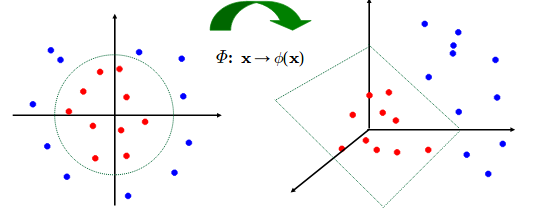
\includegraphics[width=10cm,height=12cm,keepaspectratio]{files/kernel.png}
	\caption{Transformation from one space to another using a Kernel fucntion $\phi$ (\cite{lecKernel})}
	\label{fig:kernel}
\end{figure}
The kernel trick is a mathematical tool which can be applied to any algorithm which consists of a dot product between two vectors. Kernel trick states that to compute the dot products of vectors in the higher dimensional space, a kernel function can be used directly using the lower dimensional vectors. Therefore every dot product can be replaced by this kernel function. A \textit{Kernel function}, can thus be defined as a function that takes as inputs vectors in the original space and returns the dot product of the vectors in the feature space. The feature space is usually a higher dimensional space.\\
\begin{equation}
\phi \, : \, {\rm I\!R}^n \to {\rm I\!R}^m
\end{equation}
where: m > n\\
\begin{equation}
k(\mathbf x, \mathbf y) = \phi(\mathbf x)^T \phi(\mathbf y) 
\end{equation}
\subsubsection{Which functions can act as Kernel functions?}
In order for a function to be a valid \texttt{Kernel function}, it should fulfill the \texttt{"Mercer's theorum"}. According to the Mercers' theorem, every positive definite symmetric function can be seen as a kernel function. Here a positive definite symmetric functions correspond to a "positive definite symmetric Gram matrix" which can be understood as a matrix which has all positive eigenvalues. Therefore a function which fulfill these conditions can be refereed as \textit{kernel function}.\\\\
There are many choices of the kernel function, $\mathit{k}$,which are as follows:\\
\begin{enumerate}
	\item \textbf{Linear Kernel:}
	It is the simplest type of kernel function. It can be denoted as follows:
	\begin{center}
		$\phi : \mathbf{x} \rightarrow \phi(\mathbf{x})$
	\end{center}
	\begin{center}
		where $\phi(\mathbf{x})$ is $\mathbf{x}$ itself
	\end{center}
	Thus a linear kernel can be of form:
	\begin{equation}
	k(\mathbf{x},\mathbf{y}) = (\mathbf{x}^T \mathbf{y} +1)
	\end{equation}
	Linear kernel finds its usage mostly in text classification tasks. The most important usage of this Kernel is in SVM as training a SVM with a linear kernel is much faster as compared to other kernels.
	\item \textbf{Polynomial Kernel:} 
	A polynomial kernel is a function which maps the input space into a non-linear space represented by a polynomial function. It can be denoted as follows:
	\begin{equation}
	k(\mathbf{x},\mathbf{y}) = (\mathbf{x}^T \mathbf{y} +1)^p
	\end{equation}
	\begin{center}
		where: $p$ is the degree of the polynomial.
	\end{center}
	\item \textbf{Gaussian Kernel}\\
	Also known as radial basis function kernel (RBF), it is one of the most powerful kernels. 
	Since the value of RBF kernel decreases with distance and ranges between 0 and 1 (when x = $x'$), it can be used as a similarity measure.
	\begin{equation}
	k(\mathbf{x},\mathbf{y})=\exp\left(-\frac{\|\mathbf{x}-\mathbf{y}\|^{2}}{\sigma^{2}}\right) 
	\end{equation}
	The Gaussian RBF kernel is very popular and makes a good default kernel as the feature space of this kernel has an infinite number of dimensions.
\end{enumerate}
\subsection{Kernel PCA}
Kernel Principle Component Analysis is the nonlinear form of PCA, which allows to generalize standard PCA to nonlinear dimensionality reduction. In other words, it can be referred as a non-linear dimensionality reduction technique through the use of kernel function. 
\begin{figure}
	\centering
	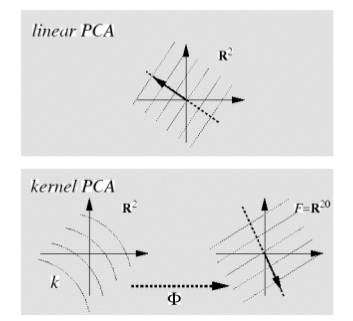
\includegraphics[width=10cm,height=12cm,keepaspectratio]{files/kernelPCA.png}
	\caption{ Kernel PCA: A nonlinear kernel function $\kappa$is used instead of the standard dot product. It implicitly perform PCA in a  possibly high-dimensional space $ F $ which is  nonlinearly related to input space. (\cite{scholkopf1997kernel})}
	\label{fig:kpca}
\end{figure}
\cite{scholkopf1997kernel} have shown that the generalization of PCA for non-linear data can be done via a kernel function.
\begin{equation}
covar = \dfrac{1}{N}\sum_{i=1}^{N}\phi(\mathbf{x}_i)\phi(\mathbf{x}_i^T)
\end{equation}
The covariance matrix in the higher dimensional space is not calculated explicitly but with using a kernel function such that: 
\begin{equation}
\kappa(\mathbf{x},\mathbf{y}) = \mathbf{\langle\phi(x),\phi(y)\rangle} =  \mathbf{\phi(x)^{T}\phi(y)}
\end{equation}
\begin{center}
	where: $\phi :{\rm I\!R}^d \rightarrow {\rm I\!R}^N $\\
	$\kappa$ is kernel function eg: radial basis function.
\end{center}
However, it is not guaranteed that the kernel matrix is centered, therefore to achieve the centered kernel matrix, \cite{scholkopf1998nonlinear} proposed:
\begin{equation}
\mathbf{\tilde{K} = K -I_NK-KI_N+I_NKI_N}
\end{equation} 
\begin{center}
	where: $\mathbf{1_N}$ is a $N\times N$ matrix with values equal to $\dfrac{1}{N}$
\end{center}
The standard steps of kernel PCA dimensionality reduction can be summarized as discussed by \cite{wang2012kernel}:
\begin{algorithm}[H]
	\caption{Kernel PCA}\label{kernelpca}
	\begin{algorithmic}[1]
		\State Construct the kernel matrix $\mathbf{K}$ from the training data set $\{\mathit{x_i}\}$ where $\mathbf{K_{ij}} = \mathit{\kappa(\mathbf{x}_i,\mathbf{x}_j)}$.
		\State Compute the kernel centered matrix  $\mathbf{\tilde{K}}$
		\State Solve $ \mathbf{\tilde{K} a}_\mathit{k} = \lambda_k N \mathbf{a}_\mathit{k}$ for the value of $\mathbf{a}_\mathit{i}$
		\State Compute  the  kernel  principal  components $y_k(\mathbf{x}) = \sum_{i=1}^{N} a_{k,i}\kappa(\mathbf{x,x}_i)$
	\end{algorithmic}
\end{algorithm}
\cite{scholkopf1997kernel} have also stated some advantages of using \textit{Kernel PCA}, for example, nonlinear principal components afforded better recognition rates than the linear ones. Another advantage is that better performance can be achieved for the nonlinear components by using more components which is not the case in the linear components. This can be used for applications such as feature extraction and data classification. 
\subsection{Artificial Neural networks and Deep Learning}
Artificial Neural Network or ANN is a term inspired by the sophisticated functionality of the human brain. In mathematical terms one might consider artificial neural networks as \textit{"universal function approximators"}.
A neural network is a collection of connected units called artificial neurons. The nodes takes the input data and perform some simple operations on the data. The output at each node is called its activation. This output can act as the input for the other nodes. Each link is also associated with a weight. This weight is assigned on the basis of its relative importance to the other inputs. A simple neuron can be represented by the \ref{fig:neuron}\\
\begin{figure}[H]
	\centering
	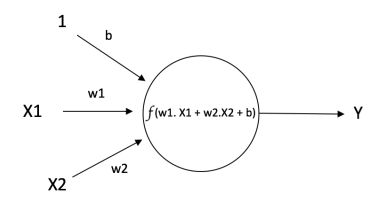
\includegraphics[width=10cm,height=12cm,keepaspectratio]{files/neuron.png}
	\caption{A single neuron with output $Y =f(w1.X1+w2.X2+b)$ (\cite{neuron})}
	\label{fig:neuron}
\end{figure}
The main aim of a neural network is to approximate some function $\mathit{f'}$. To attain such a goal, they define a mapping, $\mathbf{y} = f(\mathbf{x;w})$ and try to learn the parameters, $\mathbf{w}$, which makes the best approximation for the function $\mathit{f'}$. 
A non-linear transformation with function "$\phi$" can be applied on input $\mathbf{x}$ to extend linear models to represent nonlinear models. 
\begin{equation}
\mathbf{y} = f(\mathbf{x;w,\theta)} = \phi(\mathbf{x;w})^T \mathbf{\theta}
\end{equation}
Alternatively, \textbf{kernel trick} can also be used for such transformation. The advantage of using the neural networks is that the transformation function $\phi$ is not hard coded but can be learned and thus eliminating the need of manually engineer the function $\phi$. 	
\subsubsection{Types of Artificial Neural Networks}
\begin{enumerate}
	\item \textbf{Feedforward ANN:} 
	As the name indicates, a model is known as \textit{feed-forward neural network} when the information flows in the forward direction through a function, $f$, being evaluated from $\mathbf{x}$ through the intermediate computations and finally to the output $\mathbf{y}$. Such networks are also known as multilayer perceptrons(MLP). \\
	\begin{figure}[H]
		\centering
		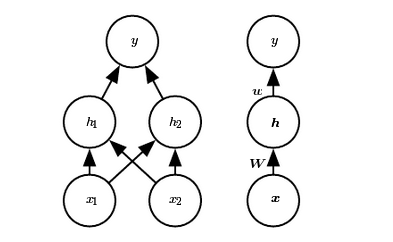
\includegraphics[width=10cm,height=12cm,keepaspectratio]{files/feedForward.png}
		\caption{Forward Neural Network (\cite{Goodfellow-et-al-2016})}
		\label{fig:fnn}
	\end{figure}
	\item \textbf{FeedBack ANN}
	In these neural networks, a feedback connection is present through which the outputs of the model are fed back into itself thus taking the previous time stamp's results into account. Such neural networks are also known as \textit{Recursive or Recurrent Neural Network}.
	\begin{figure}[H]
		\centering
		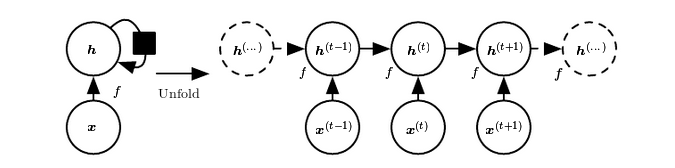
\includegraphics[width=10cm,height=12cm,keepaspectratio]{files/recurrentNN.png}
		\caption{A recurrent network with no outputs. This recurrent network just processes information from the input $\mathbf{x}$ by incorporating it into the state $\mathbf{h}$ that is passed forward through time$\mathbf{t}$. (Left) Circuit diagram. The black square indicates a delay of a single time step. (Right) The same network seen as an unfolded computational graph, where each node is now associated with one particular time instance (\cite{Goodfellow-et-al-2016})}
		\label{fig:fnn}
	\end{figure}
\end{enumerate}
\subsubsection{Design paradigms of a Neural Networks}
\begin{enumerate}
	\item \textbf{Activation function}
	The function, $f$ in figure \ref{fig:neuron} is a non-linear function and referred as an activation function. The purpose of such a function is to introduce non-linearity in the output of the neuron. There are various activation functions that can be used, some of them are represented in figure, \ref{fig:act}
	\begin{figure}[H]
		\centering
		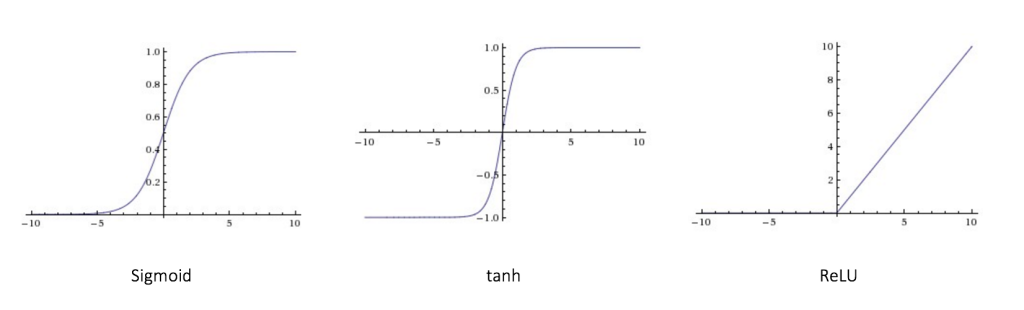
\includegraphics[width=15cm,height=25cm,keepaspectratio]{files/act.png}
		\caption{Popular activation functions generally used. (\cite{neuron})}
		\label{fig:act}
	\end{figure}
	Non linear activation functions are usually preferred because if a linear function is used then neural networks are as effective as a network with only one layer, regardless of how complex its architecture is. An activation function can also be considered as a decision making function that determines the presence of particular neural feature. Thus non-linearity is also needed in these functions because it helps the network to produce a nonlinear decision boundary via non-linear combinations of the weight and inputs.
	\item \textbf{Loss function}
	Another important design decision in neural networks, is to choose an appropriate loss function. A loss function can be seen as a function which maps a set of parameter values for this network onto some scalar value which indicates how well those parameter accomplish the task that the network intended to do. The ultimate goal is to solve the optimization problem which seeks to minimize this loss function.\\
	There are certain cases, where it is advantageous to specify a different loss for every single measurable value. This has been an active research area and there exists many types of loss functions which works better in different problem settings. The most common cost function is the Mean Squared Error (MSE) and the Cross Entropy Cost function. The latter cost function is used when working with logistic or softmax output layers. On the other hand, the mean square loss is better when solving classification problems. Other types of loss function are hinge loss, cosine proximity, sparse softmax cross entropy loss, Kullback Leibler (KL) Divergence loss.  
	\subsubsection{Solving for optimal solution for Neural Network: Back Propagation}
	One of the major difference between the linear models and neural networks is that the nonlinearity of a neural network causes the loss functions to become \textit{non-convex}. Hence there is not global minima for this loss, therefore an iterative, gradient-based optimizers method is needed to train the model. In other words, the gradient descent is used to search the local minima of the function which move in that direction in small incremental steps.
	\begin{equation}
	\mathbf{W}^{\tau+1} = \mathbf{W}^\tau - \eta \dfrac{d\mathbf{E(W)}}{d\mathbf{W}}
	\end{equation}
	\begin{figure}[H]
		\centering
		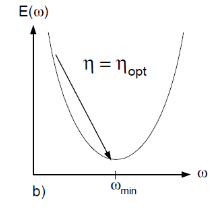
\includegraphics[width=10cm,height=5cm,keepaspectratio]{files/grad.png}
		\caption{Gradient Descent(\cite{lecun2012efficient})}
		\label{fig:act}
	\end{figure}
	This gives an optimized value, rather than the guaranteed value. Reaching the minima efficiently and in reasonable time is a very important research area. Convergence of gradient descent depends on many factors. Some of them are discussed here.\\
	\begin{figure}[H]
		\centering
		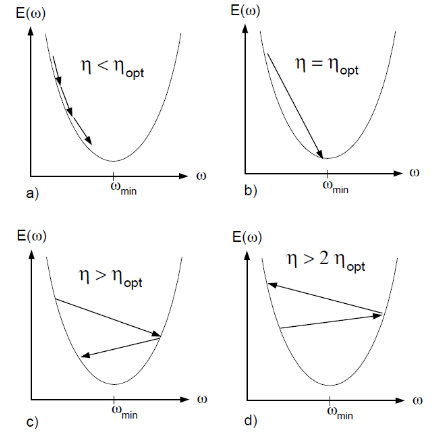
\includegraphics[width=10cm,height=15cm,keepaspectratio]{files/learningRate.png}
		\caption{Behavior for different learning rates (\cite{lecun2012efficient})}
		\label{fig:learn}
	\end{figure}
	\begin{itemize}
		\item Initialization of parameters is an important factor in determing how long the model takes to converge. Stochastic gradient descent applied to non-convex loss functions has no such convergence guarantee and hence the initial parameters should be chosen wisely for example initial parameters should be small and random values.
		\item Another factor is the how to choose the learning rate as discussed by \cite{lecun2012efficient}. Effects of choosing this factor is demonstrated in the fig, \ref{fig:learn}.
	\end{itemize}
	These techniques are important as convergence might be very slow and also sometimes lead to vanishing gradient or even exploding gradients. In such cases, clipping gradient, intelligent initialization of parameters, normalizing data and other tricks of trade makes life bit easier.
\end{enumerate}	
\section{\textit{n}-Gram Model}
There have been an increased research in Natural Language Processing which is mainly concerned with the interactions between computers and human languages. Both semantics and syntax of the language makes it understandable for humans. In language modeling, there has always been an active research for capturing both of these information. There are generally two types of \textit{n}-grams in Computational Linguistics.

\subsection{Word \textit{n}-grams}
This kind of \textit{n}-gram model is generally used in distributive word embeddings as they help in capturing semantic information in the language. These are particularly useful in learning words which are used in similar context. Variance in value of \textit{n} determines the quality of the model. 
\begin{center}
	\begin{tabular}{ c c }
		text:& to be or not to be\\
		Uni-gram:& to, be, or, not, to, be\\
		Bi-gram:& to\_be, be\_or, or\_not, not\_to, to\_be\\
		Tri-gram:& to\_be\_or, be\_or\_not, or\_not\_to, not\_to\_be\\
	\end{tabular}
\end{center}
\subsection{Character \textit{n}-grams}
The character \textit{n}-gram helps in capturing the morphological structure of the words. These are particularly helpful when dealing with morphological similar languages like Turkish or German. Therefore in such languages, one can say that the words are similar when they have a common root/morpheme. If we take the example of the English language, some of the words are formed by taking basic words and adding combinations of prefixes and suffixes to them. This can thus be considered as a good measure for similarity. 
\textit{n}-Gram is one approach to measure similarity between words  based on the common n-grams present in a word. Here \textit{n} can be 2,3,4. It algorithmically quantify the similarity between a set of strings from a finite alphabet. 
\begin{center}
	\begin{tabular}{ c c }
		text:& ankit\\
		Uni-gram:& a, n, k, i, t\\
		Bi-gram:&  \_a, an, nk, ki, it, t\_ \\
		Tri-gram:& \_an, ank, nki, kit, it\_ \\
	\end{tabular}
\end{center}
From some previous works, it can be deduced that \textit{n = 3, 4} gives the best results statistically. Example: The similarity between words "Minimal", "Minimize" is greater than the similarity between "Minimal" and "Maximize".\\
There has been a lot of work done in finding similarity between words using \textit{N}-Gram. \cite{kondrak2005n} has give a formal, recursive definitions of n-gram similarity and distance of the words. He has also proposed an efficient algorithms for computing them. The algorithm involves combining different similarities values obtained from different \textit{n}-gram models. 
We can thus select different values of \textit{n} for finding similarities based on the purpose. Uni-gram, bi-gram, tri-gram are some of the examples. One important consideration  that should be taken in account while calculating similarity is that spaces before the starting of the word and at the end of the word should also be taken in the set of \textit{n}-grams.\\
\\
\textbf{String Kernel Similarity}
One important use of \textit{n}-gram, is in computing string similarity as discussed in \cite{martins2006string} and \cite{bauc}.  In this work, we have also used \textit{n}-grams to calculate the \textit{String Kernel function}.\\
For example: If $s_1$ and $s_2$ are two words and $B_1$ and $B_2$ are their respective \textit{n}-gram sets then, a similarity function, $\mathcal{S}$, can be defined in equation, \ref{eq:sks}:\\
\begin{equation}\label{eq:sks}
\mathcal{S}(s_1,s_2) = \frac{2\times\mid B_1\cap B_2\mid}{\mid B_1 \mid + \mid B_2 \mid}
\end{equation}
and
\begin{equation}
d(s_1,s_2) = 1- \mathcal{S}(s_1,s_2)
\end{equation}
Here $d(s_1,s_2)$ can be seen as a distance measure between two words $s_1$ and $s_2$. This distance measure can then be used in a Kernel function. An example of such a kernel function is:
\begin{equation}
k(s_1,s_2) = exp\Bigg(\dfrac{-d^2(s_1,s_2)}{2\sigma^2}\Bigg)
\end{equation}
\section{Numeric Representation of Words}

\subsection{One Hot Vector Encoding}
For a vocabulary of size $\mathbf{V}$, one hot vector encoding helps in formalizing a vector of a word with the position of the word in the dictionary. Therefore a one hot vector of a word will have all "0" and at the position of the word in the dictionary, it will have a "1". The vector size is thus same as the size of vocabulary.
One hot vector encoding can also be seen as a hashing technique. This is illustrated in the following example.
\begin{center}
	For  the sentence \texttt{"the cat sat on the mat"}, one hot vector matrix will be represented as follows:
\end{center}
\begin{center}
	The dictionary of the sentence is:\\
	\{'the':0,'cat':1,'sat':2,'on':3,'mat':4\}\\
\end{center}
\begin{center}
	$\left(
	\begin{array}{ll}
	\text{the} \\
	\text{cat} \\
	\text{sat} \\
	\text{on}  \\ 
	\text{the}  \\ 
	\text{mat}  \\ 
	\end{array}%
	\right). = 
	\left( 
	\begin{array}{ll}
	\text{1 0 0 0 0} \\
	\text{0 1 0 0 0} \\
	\text{0 0 1 0 0} \\
	\text{0 0 0 1 0}  \\ 
	\text{1 0 0 0 0}  \\ 
	\text{0 0 0 0 1}  \\
	\end{array}%
	\right). $
\end{center}
As it can be inferred from the above example, such vectors only encode the information of the position of the word in the vocabulary and hence are very sparse. Such vectors are very less informative which becomes a limitation of this representation.
\subsection{Distributed Representations of Words: Word Embeddings}
To overcome the limitations of \texttt{one-hot vector}, a more informative representation is needed which can encode the information like semantic or syntactic similarities between the words. A distributed representation of words fulfills these requirements. These embeddings are captured using a "one hidden layer network architecture", such as \texttt{Continuous Bag Of Words (CBOW)} and \texttt{Continuous Skip Gram Model}.
\subsubsection{Continuous Skip Gram Model (CBOW Model)}
The model of Continuous Bag-of-Words Model(CBOW) is represented in the figure, \ref{fig:cbow_sg}. It follows a very similar approach as the feed forward NNLM proposed by \cite{bengio2003neural}. The goal of CBOW is to predict a word given a set of its context words. Context here is defined as the number of words to the left and to the right of the given word. Example of input and output with \textbf{C=1} of the model is demonstrated in the below example:\\
\textbf{Text:} \texttt{Roberta ran rings around Roman ruins.}\\
\textbf{Input and Output pair:}\\
 \texttt{(ran,[Roberta,rings]),(rings,[ran, around]), (around,[rings, Roman]),(Roman)
 	[around, ruins])...}
\begin{figure}[H]
	\centering
	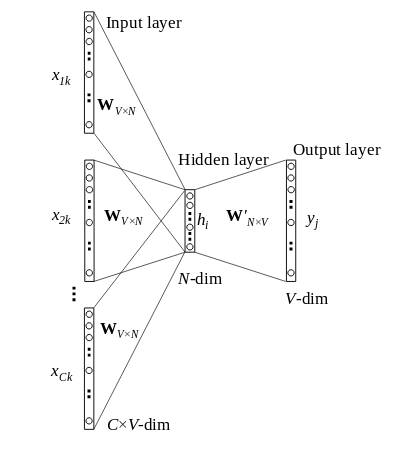
\includegraphics[width=15cm,height=12cm,keepaspectratio]{files/cbow.png}
	\caption{\textit{CBOW Model} (\cite{DBLP:journals/corr/Rong14})}
	\label{fig:cbow_sg}
\end{figure}
The model is a neural network with one hidden layer and consists of two weight matrices, $\mathbf{W_{V\times N}}$ and $\mathbf{W'_{N\times V}}$. These weights represents \textit{input word vectors}, $\mathbf{v}_w$ and \textit{output word vectors}, $\mathbf{v'}_w$. Since $\mathbf{x}$ are one-hot vector encoding for words, hence equation, \ref{eq:01} is essentially copying the corresponding row of $\mathbf{W}$ to $\mathbf{h}$. This implies that the activation function of the hidden layer units is linear. One important thing to note here is that the order of the words in context are averaged as presented in equation, equation \ref{eq:01} and hence the order of these words has no influence over the projection.
\begin{equation}\label{eq:01}
\begin{split}
\mathbf{h} & = \frac{1}{C} \mathbf{w}^T(\mathbf{x_1+x_2+...+x_C})\\
& = \frac{1}{C}(\mathbf{v}_{w_1}+\mathbf{v}_{w_2}+...+\mathbf{v}_{w_C})
\end{split}
\end{equation}
Each $\mathit{j^{th}}$, column in the matrix, $\mathbf{W'}$, of dimension ($N\times V$), is represented by the vector, $\mathbf{v'}_{w_{j}}$. This vector helps in calculating a score $\mathit{u_j}$ for each word in the vocabulary. This score is represented as:
\begin{equation}
\mathit{u_j} = \mathbf{v'}_{w_{j}}^{\mathbf{T}}\mathbf{h}
\end{equation}
This score can be used in a softmax classification model, to obtain the posterior distribution of words.
\begin{equation}
\mathit{y_j} = \mathit{p(w_j \mid w_{I,1}..w_{I,C})} = \dfrac{exp(u_j)}{\sum_{j'=1}^{V}exp(u_{j'})}
\end{equation}
This can be also represented by the following equation:
\begin{equation}\label{eq:02}
\mathit{p(w_j \mid w_{I,1}..w_{I,C})} =\dfrac{exp(\mathbf{v'}^T_{w_{j}} \mathbf{v}_{w_{I}})}{\sum_{j'=1}^{V}exp(\mathbf{v'}^T_{w_{j'}} \mathbf{v}_{w_{I}})}
\end{equation}
The model is thus trained by maximizing its log-likelihood on the training set or minimizing the negative log-likelihood of:
\begin{equation}
E = - \log p(w_j\mid w_{I,1},...,w_{I,C})
\end{equation}
The goal now is to optimize the weights so as to improve (in this case, maximize) the objective function in equation, \ref{eq:02}. This is done by deriving the gradient of the loss with respect to the embedding parameters/weights. An update to the embeddings is made by taking a small step in the direction of the gradient. When this process is repeated over the entire training set, this has the effect of moving the embedding vectors around for each word until the model is successful at discriminating real words from noisy words.
\subsubsection{Skip-Gram Model} 
Skip gram model is simpler model when compared to Continuous Bag of Words. It's goal is opposite of that of a CBOW model. In other words, at the output layer, instead of getting one multinomial distribution, there are $C$ multinomial distributions of the words. For example, using a window size of 1, we then have the dataset with context words one left and one right.\\
The dataset consists of a context and target pair. For example as shown below: \cite{tensorflow2015-whitepaper}:\\\\
\textbf{Text:} 
\texttt{Roberta ran rings around Roman ruins.}\\
\textbf{Input and Output pair:}
\texttt{([Roberta,rings], ran),([ran, around],rings), ([rings, Roman],around),([around, ruins],Roman)...}
\\\\
It is worth noting that larger the context window, \textbf{C}, more are training examples and thus can lead to a higher accuracy, at the expense of the training time.\\
\begin{figure}[H]
	\centering
	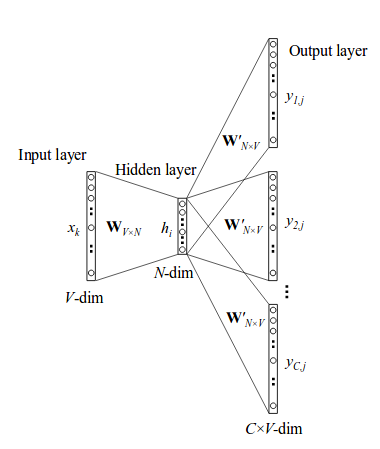
\includegraphics[width=15cm,height=12cm,keepaspectratio]{files/skip-gram.png}
	\caption{\textit{Skip-Gram Model} (\cite{DBLP:journals/corr/Rong14})}
	\label{fig:skip_sg}
\end{figure}
The scoring function remains same in this model as the CBOW model. Skip gram model performs better than the CBOW model, when it come across a rare word but is slower to train. This can be accounted to the fact that it does not average the embedding vectors. It seems like the model can learn better representations for the rare words when their vectors are not averaged with the other context words in the process of making the predictions.\\\\
In both the models, the quality of the word vectors increases significantly with amount of the training data. Both the models are widely popular because of their simple structure and use of a shallow network and have their own individual advantages. The skip gram model takes longer than CBOW model to get trained but performs much better on semantic tasks. Whereas CBOW model works better on syntactic tasks. The choice of the model depends on the problem domain and datasets.
\subsubsection{Optimizing Computational Efficiency}
In both the models proposed by \cite{mikolov2013efficient}, the output involves applying a \texttt{softmax function} represented in equation, \ref{eq:02}. If analyzed closely, it turns out to be computationally very expensive since the denominator of the \texttt{softmax function} is a dot product of the word with \textit{all the words in the vocabulary}. Thus there is a dire need for optimizing this function.
There are two approaches for optimizing the algorithms discussed above.
\begin{enumerate}
	\item \textbf{Hierarchical Softmax: }
	Hierarchical softmax, proposed by \cite{morin2005hierarchical}, is an approximation of softmax inspired by binary trees. It converts a flat softmax layer into a hierarchical layer that has the words as leaves and each node, explicitly represents the relative probabilities of its child nodes. Therefore, each word, $\textit{w}$ can be reached by an appropriate path from the root of the tree. The probability of a word, being the output word can be represented as:
	\begin{equation}
	p(w = w_O) = \prod_{j=1}^{L(w)-1} \sigma(\llbracket n(w,j+1) = ch(n(w,j))\rrbracket \cdot \mathbf{v'}^T_{n(w,j)}\mathbf{h})
	\end{equation}
	where:
	\begin{enumerate}
		\item $ch(n)$ is the left child of unit $n$.
		\item $\mathbf{v'}^T_{n(w,j)}$ is the vector representation of the inner units $n(w,j)$ .
		\item $\mathbf{h}$ is the output of the hidden layer.
		\item $\llbracket f\rrbracket$ is a special function which gives $1$ or$-1$ for condition being true or false. 
	\end{enumerate}
	The structure of the tree used by the hierarchical softmax has a considerable effect on the performance. \cite{mikolov2013distributed} used binary Huffman tree.
	\item \textbf{Negative Sampling: }
	Another optimization technique used in \cite{mikolov2013distributed} is negative sampling. The idea behind this approach is very straight forward when compared to hierarchical softmax. Essentially, the probability for selecting a word as a negative sample is related to its frequency, with more frequent words being more likely to be selected as negative samples. The Negative sampling (NEG) is defined by the objective function:
	\begin{equation}
	E = -\log \sigma(\mathbf{v'^T_{w_O}}\mathbf{h}) - \sum_{w \in \mathcal{W}_{neg}}\log\sigma(-\mathbf{v'}_{wj}\mathbf{h})
	\end{equation}
	where: 
	\begin{enumerate}
		\item $w_O$ is the output vector from the positive sample.
		\item $\mathcal{W}_{neg}$ are the negative sample set of words that are sampled from the noise distribution, $P_{n}(w)$ 
	\end{enumerate}
\end{enumerate}
	\chapter{Related Work}
\label{cha:relwork}
\section{Word Embeddings}
Word embeddings is a collective term which can best be described as a set of language modeling and feature learning techniques in natural language processing (NLP). Using these techniques, words or phrases from the vocabulary, are mapped to vectors of real valued numbers. 
The term word embeddings was originally coined by \cite{bengio2003neural}. It can be seen as a function which captures the important statistical characteristics of the distribution of sequences of words, allowing one to make probabilistic predictions of the next word given the current word. There have been a lot of active research conducted in this area. Some of the major results which revolutionized this field are discussed in this section. Every method discussed in this section for generating such vector representations is generally based on Neural Networks architecture.  
\subsection{Neural Probabilistic Language Model}
\cite{bengio2003neural} proposed a neural distributed representation for words. The proposed model allows each training sentence to inform the model about an exponential number of semantically neighboring sentences. The model is a feed-forward neural network, which mainly consists of a hidden layer and helps in predicting the next word in a sequence. They stated that the distributed representations for symbols could be combined with neural network probability predictions. 
\begin{equation}
\mathbf{J}_\theta = \frac{1}{T}\sum_{t=1}^{T}log f(w_t,w_{t-1},..,w_{t-n+1})\\.
\end{equation}
where: $f(w_t,w_{t-1},..,w_{t-n+1})$ is computed by the softmax applied in the last layer
\begin{figure}[H]
	\centering
	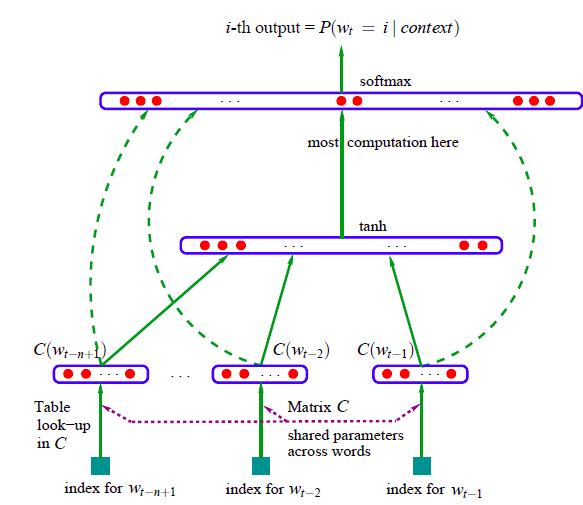
\includegraphics[width=15cm,height=12cm,keepaspectratio]{files/npmodel.png}
	\caption{Neural Probabilistic Model (\cite{bengio2003neural})}
	\label{fig:npm}
\end{figure}
The first layer is an embedding layer, which generates word embeddings by multiplying an index vector with a word embedding matrix. In the middle, there are one or more layers that produce an intermediate representation of the input. Such a layer may be a fully-connected layer that applies a non-linearity to the concatenation of word embeddings of $n$ previous words thus taking context in consideration. The final layer is a softmax layer which produces a probability distribution over words in the vocabulary, $\mathbf{V}$ and thus supplying with a prediction of the word.\\
\cite{bengio2003neural} reported that their approach has achieved significant improvement on state-of-the-art n-gram models, meanwhile taking the advantage of longer contexts.

\subsection{Distributive Word Representation}\label{w2v}
In their paper, \cite{mikolov2013efficient} introduced a technique to learn word vectors from a huge data corpus which contains billions of words. They have proposed two new model architecture for learning the distributed representation of the words. Besides the models, \cite{mikolov2013efficient} also proposed some techniques to determine similarity measures between words. The two models are known as Continuous Bag-of-Words Model and Continuous Skip-gram Model. The models are trained on dataset of size $N$ with vocabulary size $V$ to generate the vectors of dimension $D$. 
A brief description of these models are as follows:
\subsubsection{Continuous Bag-of-Words Model (CBOW)}
The model, introduced by \cite{mikolov2013efficient}, tries to predict the current word based on its context words. This model is very similar to the feedforward NNLM, but uses a continuous distributed representation of context instead of bag-of-words. They also stated that the training time complexity of the model is:
\begin{equation}
Q = N \times D + D \times \log_2(V)
\end{equation}
\subsubsection{Continuous Skip-gram Model}
Another model proposed by \cite{mikolov2013efficient}, is similar to CBOW but it tries to maximize classification of a word based on the words in the same sentence. In other words, the model predicts the context words given their center word. Here distance of words to the input word, represented by $C$, also comes in play. This distance is important since the more distant words are less related to the center word. So one can assign less weight to distant context words thus helps to attain better context words. They also stated that the training time complexity of the model is:
\begin{equation}
Q = C \times (D+D\times\log_2(V))
\end{equation}
Both the models became very popular because of their simple and shallow architecture. They are easy to train and generate high quality word vectors.
\subsection{Global Vectors(gloVe)}
In this paper, \cite{pennington2014glove}, proposed an alternative model to generate word embeddings. They proposed to use the statistics of word co-occurrences in a corpus. They tried to explore the relationship between words using these statistics. They referred to the model as GloVe, "Global vectors", as the model explores the global corpus statistics.\\
\\
It is a log-bilinear model with a weighted least-squares as an objective function. The main idea that the model follows is to find the ratios of word-word co-occurrence probabilities. These ratios have the potential to encode some form of meaning. In other words, similar meaning words have a high ratio of co-occurrence.\\
The authors reported that the model performed better than the state of art models for word analogy, word similarity and named entity recognition tasks. The model introduced a new weighted least square regression model. This is done by using a weighing function $\mathit{f(\mathbf{X}_{ij}})$ in cost function.
\begin{equation}\label{eq:J}
\mathit{J = \sum_{i,j=1}^{v} f(X_{ij})(w_i^T \tilde{w_j}+b_i+\tilde{b_j}-log X_{ij})^2}
\end{equation}
In this equation, \ref{eq:J},\\
$\mathbf{\mathit{X_{ij}}}$ denotes number of times word \textit{j} occurs in context of word \textit{i}\\
$\mathit{w \in \mathbf{R}^d}$ are word vectors.\\
$\mathit{\tilde{w} \in \mathbf{R}^d}$ are separate context word vectors.\\ 
$\mathit{b_i, \tilde{b_j}}$ are biases.\\
$\mathbf{V}$ is the vocabulary size.\\
$\mathit{f(x)}$ function that worked well in this model is:
\begin{center}
	$$
	f(x) = \left\{
	\begin{array}{ll}
	(x/x_{max})^\alpha & \quad x < x_{max} \\
	1 & \quad otherwise
	\end{array}
	\right.
	$$
\end{center}
\subsection{Word vectors using FastText}
The approach followed in this technique is the most related approach to our proposed model in this thesis. \cite{bojanowski2016enriching} proposed a model which is basically an extension of skip-gram model, \cite{mikolov2013efficient}. In this approach, the model learns the representations of sub words in addition to the words in the vocabulary. Thus the main focus of this approach is to include the morphology of words.\\
The model used in this approach is also known as Sub-word model. The main difference between this model and the skip gram model is the scoring function \textit{s}. This different scoring function, takes into account the morphological information of the words.
Each word is represented as a bag of character \textit{n}-gram. The word \textit{w} is also considered in the set. The example for the set for the word "machine" with \textit{n} = 3 include:
\begin{center}
	$\mathit{<ma, mac, ach, chi, hin, ine, ne>, <machine>}$
\end{center}
The vector for the word \textit{w} represented by $\mathbf{z_{\mathit{g}}}$ to each $\mathit{n}$-gram $\mathit{g}$ will have scoring function:
\begin{equation}
\mathit{s(w,c)} = \sum_{g\in \mathcal{G}_{\mathit{w}}} \mathbf{z}^T_{\mathit{g}}\mathbf{v}_{\mathit{c}}
\end{equation}
This is a very simple model which allows sharing the representation across words. Such approaches help in learning vector representation of rare words.\\
One drawback in this approach is that training is slower than the training of a skip gram model. On the other hand, it has also been reported that the morphological information significantly improves the syntactic tasks, as the accuracy surpassed the base line. The performance of proposed model seems to quickly saturate where as the CBOW's performance improved significantly when the data size is increased. But the most important result from the proposed approach is that very good word vectors are generated using a very small training dataset. 

	\chapter{Approach}
\label{cha:approach}
In this chapter, we will discuss in detail, the process of applying the Kernel PCA on different text data-sets and how to obtain the word embeddings using these KPCA embeddings in the skip gram model. Using this approach, we can thus make use of morphological similarities to learn semantic and syntactic similarities between the words. We will be using our approach to generate word embeddings for both morphological language, German as well as non-morphological language, English. There are many datasets available at our disposal for exploring various text analysis problems in both of these languages. We will be mainly working with \texttt{text8}, \text{wikidump2016} and \texttt{20News group} datasets for English and \texttt{news.2013.de} for German.

\section{Kernel Principal Component Analysis on Strings}\label{secKPCA}
Kernel Principal Component Analysis is a powerful algorithm in the field of machine learning. When applied, it helps in solving non-linear clustering problems in a higher dimensional space. In the following section, we will be discussing about applying Kernel PCA on "text data". As discussed in earlier chapters, when we delve into the text mining, we need word vectors to be represented in a vector space. It is very intuitive to say that since the vocabulary is quite large, we need the representation of words to be in a higher dimensional space so that we can easily represent words and the relationship them. Hence making clustering problem solvable. Kernel PCA is very helpful as it enables us to achieve this goal without explicitly working in a high dimensional space.\\
Since our goal is to cluster morphological similar words together, in the first step, we start with computing the \texttt{String similarity} between words. This similarity is computed by a function which takes the number of common \textit{n}-grams between two strings in the given vocabulary, $\mathbf{V}$. We also know that if two words have lot of \textit{n}-grams in common, then there is a high probability that these words will lie close to each other in the feature space. One such example of the similarity function is represented in the equation, \ref{eq1.1}.
 \begin{equation}\label{eq1.1}
 \mathcal{S}(s_1,s_2) = \frac{2\times\mid B_1\cap B_2\mid}{\mid B_1 \mid + \mid B_2 \mid}
 \end{equation}
 In the above equation, \ref{eq1.1}, $\mathcal{S}$ represents the similarity function computed between the words, $s_1$ and $s_2$. $B_1$ and $B_2$ are the set of \textit{n}-gram of these words. Given the vocabulary, $\mathbf{V}$, we can compute this similarity function of every word in $\mathbf{V}$ and thus obtain a similarity matrix, $\mathbf{S}$ of shape $V\times V$.
 The next step is to cluster the similar words together. Here kernel PCA comes into play. We kernelize the similarity matrix using the non-linear kernel function, $\mathcal{K}$, which generates a Kernel matrix $\mathbf{K}$ of shape $V\times V$.\\
  For applying this algorithm, choosing an appropriate kernel function is very important since this function will determine the dimension and hyperplane where clustering can be achieved. There are many kernel functions available such as Logistic kernel,  Epanechnikov kernel, Cosine kernel, Gaussian kernel and Polynomial kernel of degree, p. Clustering of words works best in languages like \textit{German} and \textit{Turkish} since the words with similar meaning have same morphemes. Because of the fact that the Gaussian kernel function works in an infinite dimensional space, it becomes a very common choice for solving such problems. Clustering using Gaussian kernel PCA is demonstrated in figures \ref{fig:kgaussianen} and \ref{fig:kgaussiande}.\\
  \begin{figure}[H]
  	\centering
  	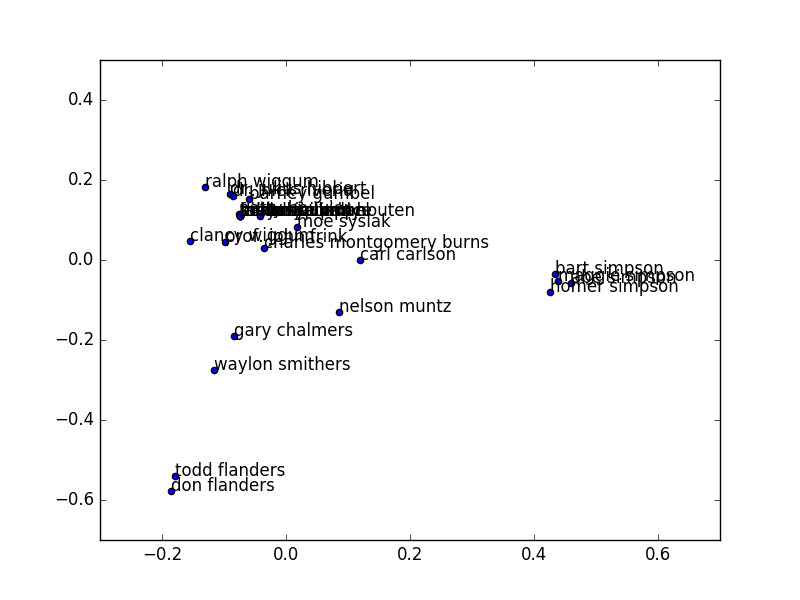
\includegraphics[width=15cm,height=12cm,keepaspectratio]{files/KERNELPCA/gaussianN3en.png}
  	\caption{Kernelized PCA using Gaussian kernel on English words using \textit{n}-grams similarity where \textit{n}=3}
  	\label{fig:kgaussianen}
  \end{figure}
   The resulting kernel matrix can be seen as vectors in a very high dimensional space. To visualize these vectors in lower dimensional space, we need to select $d$ eigenvectors of this Kernel matrix, $\mathbf{K}$. By selecting $d$ eigenvectors($\mathbf{v_d}$) corresponding to the \textit{first} $d$ eigenvalues($w_d$), we can generate a matrix $\mathbf{P}$, known as the "Projection Matrix". We should also note that selecting eigenvectors corresponding to the first $d$ eigenvalues is important because this makes sure that we have maximum variance and thus do not loose any vital information.
   \begin{equation}
   \mathbf{P} = \big[\frac{\mathbf{v_1}}{w_1},...,\frac{\mathbf{v_d}}{w_d}\big]
   \end{equation}
   The KPCA embeddings, $\mathbf{e}$ of each word in the given vocabulary, $V$ can be computed by projecting the kernel matrix row of the corresponding word on the projection matrix.
   \begin{equation}
    \mathbf{e}= \mathbf{P}^T \mathbf{k}
   \end{equation}
   where: 
   \begin{enumerate}
   	\item $\mathbf{e}$ is each row in the vector embeddings, $\mathbf{W}$.
   	\item $\mathbf{k}$ is the row of kernel matrix $\mathbf{K}$.
   \end{enumerate}
   
  \begin{figure}[H]
 	\centering
 	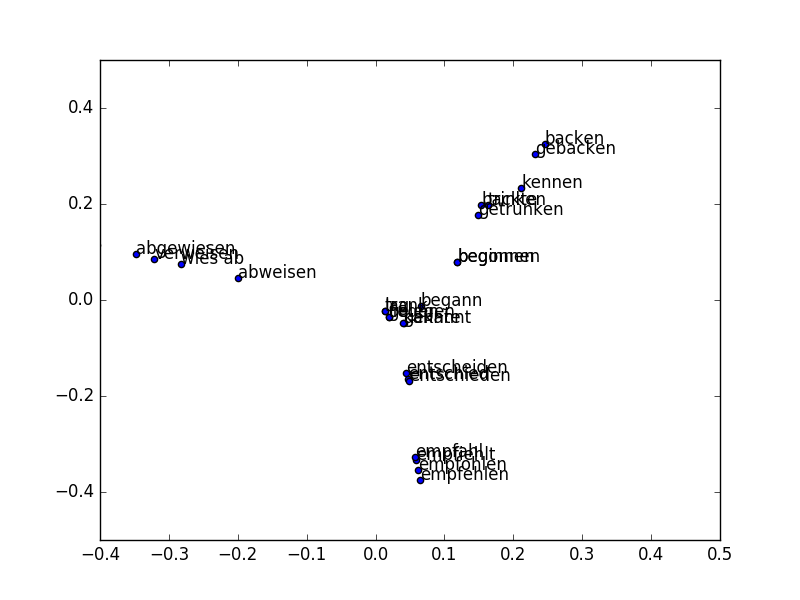
\includegraphics[width=15cm,height=12cm,keepaspectratio]{files/KERNELPCA/gaussianN3de.png}
 	\caption{Kernelized PCA using Gaussian kernel on German words using \textit{n}-grams similarity where \textit{n}=3}
 	\label{fig:kgaussiande}
 \end{figure}
Thus we can generate the "KPCA embeddings of dimension $\mathit{d}$" of a set of words. The beauty of this method is that it can be applied to any kind of non-numeric data. 
\section{Word vectors using Kernel PCA and Skip-Gram model}
 In this section, we will explore the idea of improving the word2vec skip-gram model by using word embeddings generated from Kernel PCA (KPCA embeddings). We propose an extension to the skip-gram model by feeding the model with these embeddings. The main motivation behind the approach is to use the \textit{root/morpheme} information encoded in the structure of the word, which is not considered by the word2vec models. Similar to the skip-gram model, our model also follows, an unsupervised approach for learning word embeddings. The key difference is that we are feeding the network, explicitly with the morphological similarities learned using KPCA. Hence we can say that our model uses the semantic, syntactic and morphological information in the words and the text to generate better word vectors.
 \subsection{Pre-processing the dataset}
 We are using different data-sets like Text8, 20 Newsgroups dataset, enWiki2016 dump, news.2013.de.shuffled.corpus for generating and for evaluating KPCA word embeddings. Every dataset is a collection of web articles crawled from news websites or Wikipedia. These raw text corpuses have a large amount of irrelevant text which we do not want our network to learn. Such text includes capitalization, punctuation, foreign text, tables, markup, formatting, hypertext links, and XML structure such as timestamps, authorship, and comments. This preprocessing step help us to clean the text by removing all the convert to lowercase letters and spaces, spell digits. Thus we need to filter out the junk and generate readable English.\\
 Text8 corpus is a cleaned Wikipedia text and can be used directly but we need to clean the other datasets. Text8 corpus is generated using the preprocessing script by \textit{Matt Mahoney} \footnote{\url{http://cs.fit.edu/~mmahoney/compression/text.html/}}.The script removes any text that would not be visible on the Wikipedia website besides removing the punctuations. When the text is reduced to only letters, digits, and nonconsecutive spaces, the resulting text is about 70\% of the original size. This is expanded to 74\% after spelling out digits (a common technique in speech models).\\ 
 For German text corpus, we need to perform some additional preprocessing steps. German words consist of umlauts which need to be transformed. 
 \begin{center}
 	 For example: {\"a} -> ae and \ss -> ss.
 \end{center}
 At the end, the data has to be stored in a text file or to be supplied in a continuous stream with each sentence per line with each line, being UTF-8 encoded strings/tokens separated by spaces. This file can now be used to construct a vocabulary and to train any model for text mining problems.
 \subsection{Implementing Kernel PCA on words in a vocabulary}\label{sub:vw}
 After cleaning the text corpus, we need to generate the vocabulary from this dataset. The major challenge is how to deal with a huge vocabulary. For applying Kernel PCA, we need to find the eigenvalues and eigenvectors of the Kernel matrix which is used to generate Kernel PCA embeddings. Since this computation is quite expensive and has to be done on the whole vocabulary so it is better to select an optimal subset of vocabulary to generate \textbf{Projection matrix} which can then be used to generate KPCA word embeddings for out-of-vocabulary words. The vocabulary is generated from most frequently used in the text corpus. Therefore the vocabulary consists of most frequently occurring, $\mathbf{V}$, words. In this work, we have also tried to evaluate the performance of the model with different vocabulary sizes.\\ 
 %As per \footnote{http://www.cs.trincoll.edu/~crypto/resources/LetFreq.html}, the %average length of English words is 4.5 letters, so we created a vocabulary of %words of length between 4 and 8. This created a vocabulary of size, represented %by $\mathbf{V'}$.
\begin{center}
Here $\mathbf{V}$ sizes used are 20,000 words, 30,000 words, 118,000 words.
\end{center}
 Following the steps mentioned in \ref{secKPCA} to compute the Projection matrix and Kernel PCA embeddings of dimension, $d$ for the words in the vocabulary.
 
 \subsection{Implementing Kernel PCA on out-of-vocabulary words}\label{oov}
 This step is quite straightforward to implement once we have the projection matrix of the vocabulary words. The projection matrix can be used to generate the KPCA vectors for the words which are not present in the vocabulary. By using this step, we can increase our vocabulary size for training data-sets with large vocabulary or get KPCA vectors for out of vocabulary words.\\
 
 For any word $s_n$, which is not in the vocabulary $\mathbf{V}$, we need to compute the kernel vector of dimension $\mathbf{d}$, with respect to all the words in the vocabulary. To compute the KPCA vector of $s_n$, we then project its kernel vector on the projection matrix, demonstrated in equation \ref{eq:4.4}:
 \begin{equation}\label{eq:4.4}
 	\mathbf{e}_n =\mathbf{P}^T \mathbf{k}_n
 \end{equation} 
 where:
 \begin{equation}
	 \mathbf{k}_n = \mathcal{K}(\mathcal{S}(s_n,\mathbf{V}))
 \end{equation}
This also helps in overcoming the disadvantage of word2vec model which excludes all the words with low-frequency count or may not be present in the dataset. At this stage, we can compute KPCA word embeddings for any of the Out-of-Vocabulary words. We should also note that these KPCA word vectors are only morphologically similar. We need to train them using a skip gram model to include semantic and syntactic similarities.

\subsection{Implementing word2vec model(Skip gram) with KPCA Embeddings in Tensor flow}
The major goal of word2vec models is to learn a numerical embeddings space of a vocabulary from a very large dataset. This results in similar words ending up close to each other in that feature space. As we have discussed in earlier chapter \ref{w2v}, we know that skip-gram model tries to learn the relationship between words through the context in which they are used. In simple terms, \texttt{a word is best known by the company it keeps"}. To understand this we can look at the following example:
 \begin{enumerate}
 	\item usa is a developed nation
 	\item germany is a developed nation
 \end{enumerate}
 When training the model with these two sentences, we have two batches, (input:usa, output: nation) and (input:germany, output: nation) for the respective sentences. When trained with these batches, the model will eventually be forced to understand that, "usa" and "germany" both are related to word "nation", thus placing usa and germany closely in the embedding space.\\
 The quality of word embeddings trained using "skip-gram" also depends on the size of the data-set used for training. It should be noted that the state of the art, the \texttt{pre-trained GoogleNews-vectors of dimension 300}, are trained on \texttt{$100$ billion} words dataset and took around \texttt{9 hours} for training which was done in parallel. This asserts that although the model is very simple and shallow, we still need a "very large dataset" to generate meaningful word embeddings. Even after training on such a huge dataset, we need very high dimensional word vectors to answer "very subtle" semantic relationships between words, such as a city and the country it belongs to.\\\\
 On the implementation side, skip-gram model makes use of \textit{One-hot vector} of the target word at the input layer. This vector has $\mathbf{V}$ components (one for every word in our vocabulary) and contains \texttt{"1"} in the position corresponding to the target word in the vocabulary, and \texttt{"0s"} in all of the other positions in the vocabulary and thus is very sparse and less informative. If we take \texttt{dot product} of this vector, dim $1\times V$ with the weight/embedding matrix, dim $V \times d$, it will effectively selects the matrix row corresponding to the value \texttt{"1"} in the vector. This means that the hidden layer of this model is really just operating as a \textit{"lookup table"}. There is no activation function used in the hidden layer. Hence the output of the hidden layer is just the "word vector" for the input word. This word vector is then gets fed to the output layer. The output layer is a softmax regression classifier, which helps to find the probability that a randomly selected nearby word is that vocabulary word.\\\\
The main goal of our approach is to be able to train a skip gram model using the \texttt{very basic parameters} with KPCA word embeddings, generated using the steps explained in sections \ref{sub:vw} and \ref{oov}, as the input vectors. In our model, \textbf{KPCA Skip gram model}, we tried to answer the following concerns,:
 \begin{enumerate}
 	\item Can we train a skip gram model with less epochs and still get fair quality of word embeddings?
 	\item Can we generate word embeddings on relatively smaller data set?
 	\item How fast can the network learns semantic and syntactic similarity?
 	\item Can we improve word embeddings for morphological languages?
 \end{enumerate} 
 The motivation behind these goals is that words which are having same root/morphemes are usually used in same context. This is especially true when the language is morphologically rich, like German. Therefore semantic and morphological similarity converges for most of the words and hence our model should be more efficient than the skip gram model. Since we are feeding the network with already trained morphological similarity vectors, we should be able to train our network on a relatively smaller dataset without effecting the quality of word embeddings.\\
 We are using the tensorflow skip gram word2vec implementation \footnote{https://www.tensorflow.org/tutorials/word2vec} in which we modify the word embeddings to \texttt{the Kernel PCA embeddings} thus the input to the network becomes KPCA vectors of the words.\\
 The following example demonstrates our model's implementation:\\
 If we consider the sentence:
 \begin{center}
 	\texttt{"the first principle is that you must not fool yourself"}
 \end{center}
 In the given sentence, if the target word is: \texttt{("principle")}, then we define a set of parameters for the model to be trained, 
 \begin{enumerate}
 	\item \textit{skip window} denotes the number of words back and forth from the target word. In this example if skip window = 2 then, ['The', 'first', 'principle', 'is',' that'] will be inside the window.
 	\item \textit{num skips} denotes the number of different output words that will be picked within the span for a single word. 
 	\item \textit{batch size} denotes the number of input and output pairs in one pass of forward and backward propagation. In our model, the batch size is of 128 words
 	\item \texttt{epoch} Number of times the model sees the whole data set. We are training our model for 1 epoch.
 	\item \texttt{Number of steps} This number depends on the data set size and batch size. If the dataset is of \texttt{$1000$} words and batch size is defined as \texttt{$500$} then in 1 epoch there are 2 steps to get the model trained. We have tracked results during various steps during training to see how well and quickly our model learns word vectors.
	\item NegExample denotes the number of negative examples to sample for each positive example. We are training our model with NegExample = 64.
	\item Embedding dimension defines the dimensionality of each word vector. In our model we are working in dimension = 128 and 300
	\item Vocabulary is the set of top \textbf{V} most frequent words, from the data set on which we are training our model. 
 \end{enumerate}
  The important thing to understand is that we are using numerical representations for the words. In order to do this, we will assign a unique ID to the unique words. These IDs corresponds to the index of word in the dictionary, hence act as a lookup.\\
 If we consider the above example, our dictionary will be:
 \begin{center}
  \texttt{\{"the":0,"first":1,"principle":2,"is":3\}}, so on.
\end{center}
   The input data becomes the list of indexes from the dictionary,  \texttt{[0,1,2,3,4,5,6,7...]}. This kind of input: output format helps in looking up the corresponding KPCA word vectors without explicitly using one-hot vector encoding. On this input data, the model generates batches and labels and get trained using these batches and lables\\
 We trained models on both languages: \texttt{German} and \texttt{English}.\\
 We also tinkered with the following parameters of our model for training, to see their effects on our model's performance:
 \begin{enumerate}
 	\item Dimension of input vectors, $d$
 	\item Vocabulary size, $V$
 	\item Dataset size
 \end{enumerate}
 \subsection{Results of KPCA Skip gram Model}
 When we trained our model using KPCA embeddings on a skip gram model, we get very interesting results for both morphological language, German and non-morphological language, English. To check the quality of the embeddings, the word vectors are projected on a 2-dimensional space using t-SNE. These embeddings are generated in just 40,000 steps, so that we can get an intuition about how quickly our model is learning word vectors. When figure \ref{fig:t1sne} is analyzed closely, we realize that our model tried to learn both semantic and morphological similarity between the words. This can be seen in figure \ref{fig:focusOfkpcaSm}, where we magnify some clusters formed in t-SNE in figure \ref{fig:t1sne}. In the figure \ref{fig:focusOfkpcaSm}, we can clearly see that semantically similar words like \texttt{"first"}, \texttt{"third"} got clustered together even when they are not morphologically similar where as words like \texttt{"weapons"} and \texttt{"weapon"} which would be clustered together from the first step, remain clustered.
\begin{figure}[H]
	\centering
	\subfloat[]{%
		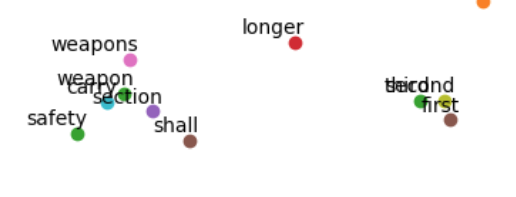
\includegraphics[width=5cm,height=2cm]{files/M128smallnews/4.png}%
		\label{fig:left}%
	} 
	\subfloat[]{%
		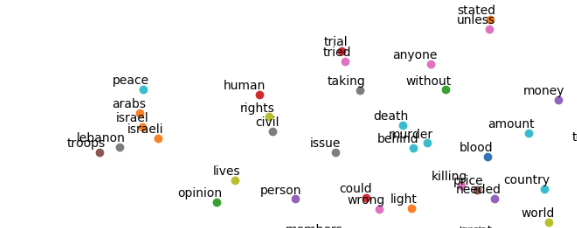
\includegraphics[width=5cm,height=2cm]{files/M128smallnews/2.png}%
		\label{fig:middle}%
	}
	\caption{Clusters of from figure, \ref{fig:t1sne}}
	\label{fig:focusOfkpcaSm}
\end{figure}
 \begin{figure}
  	\centering
  	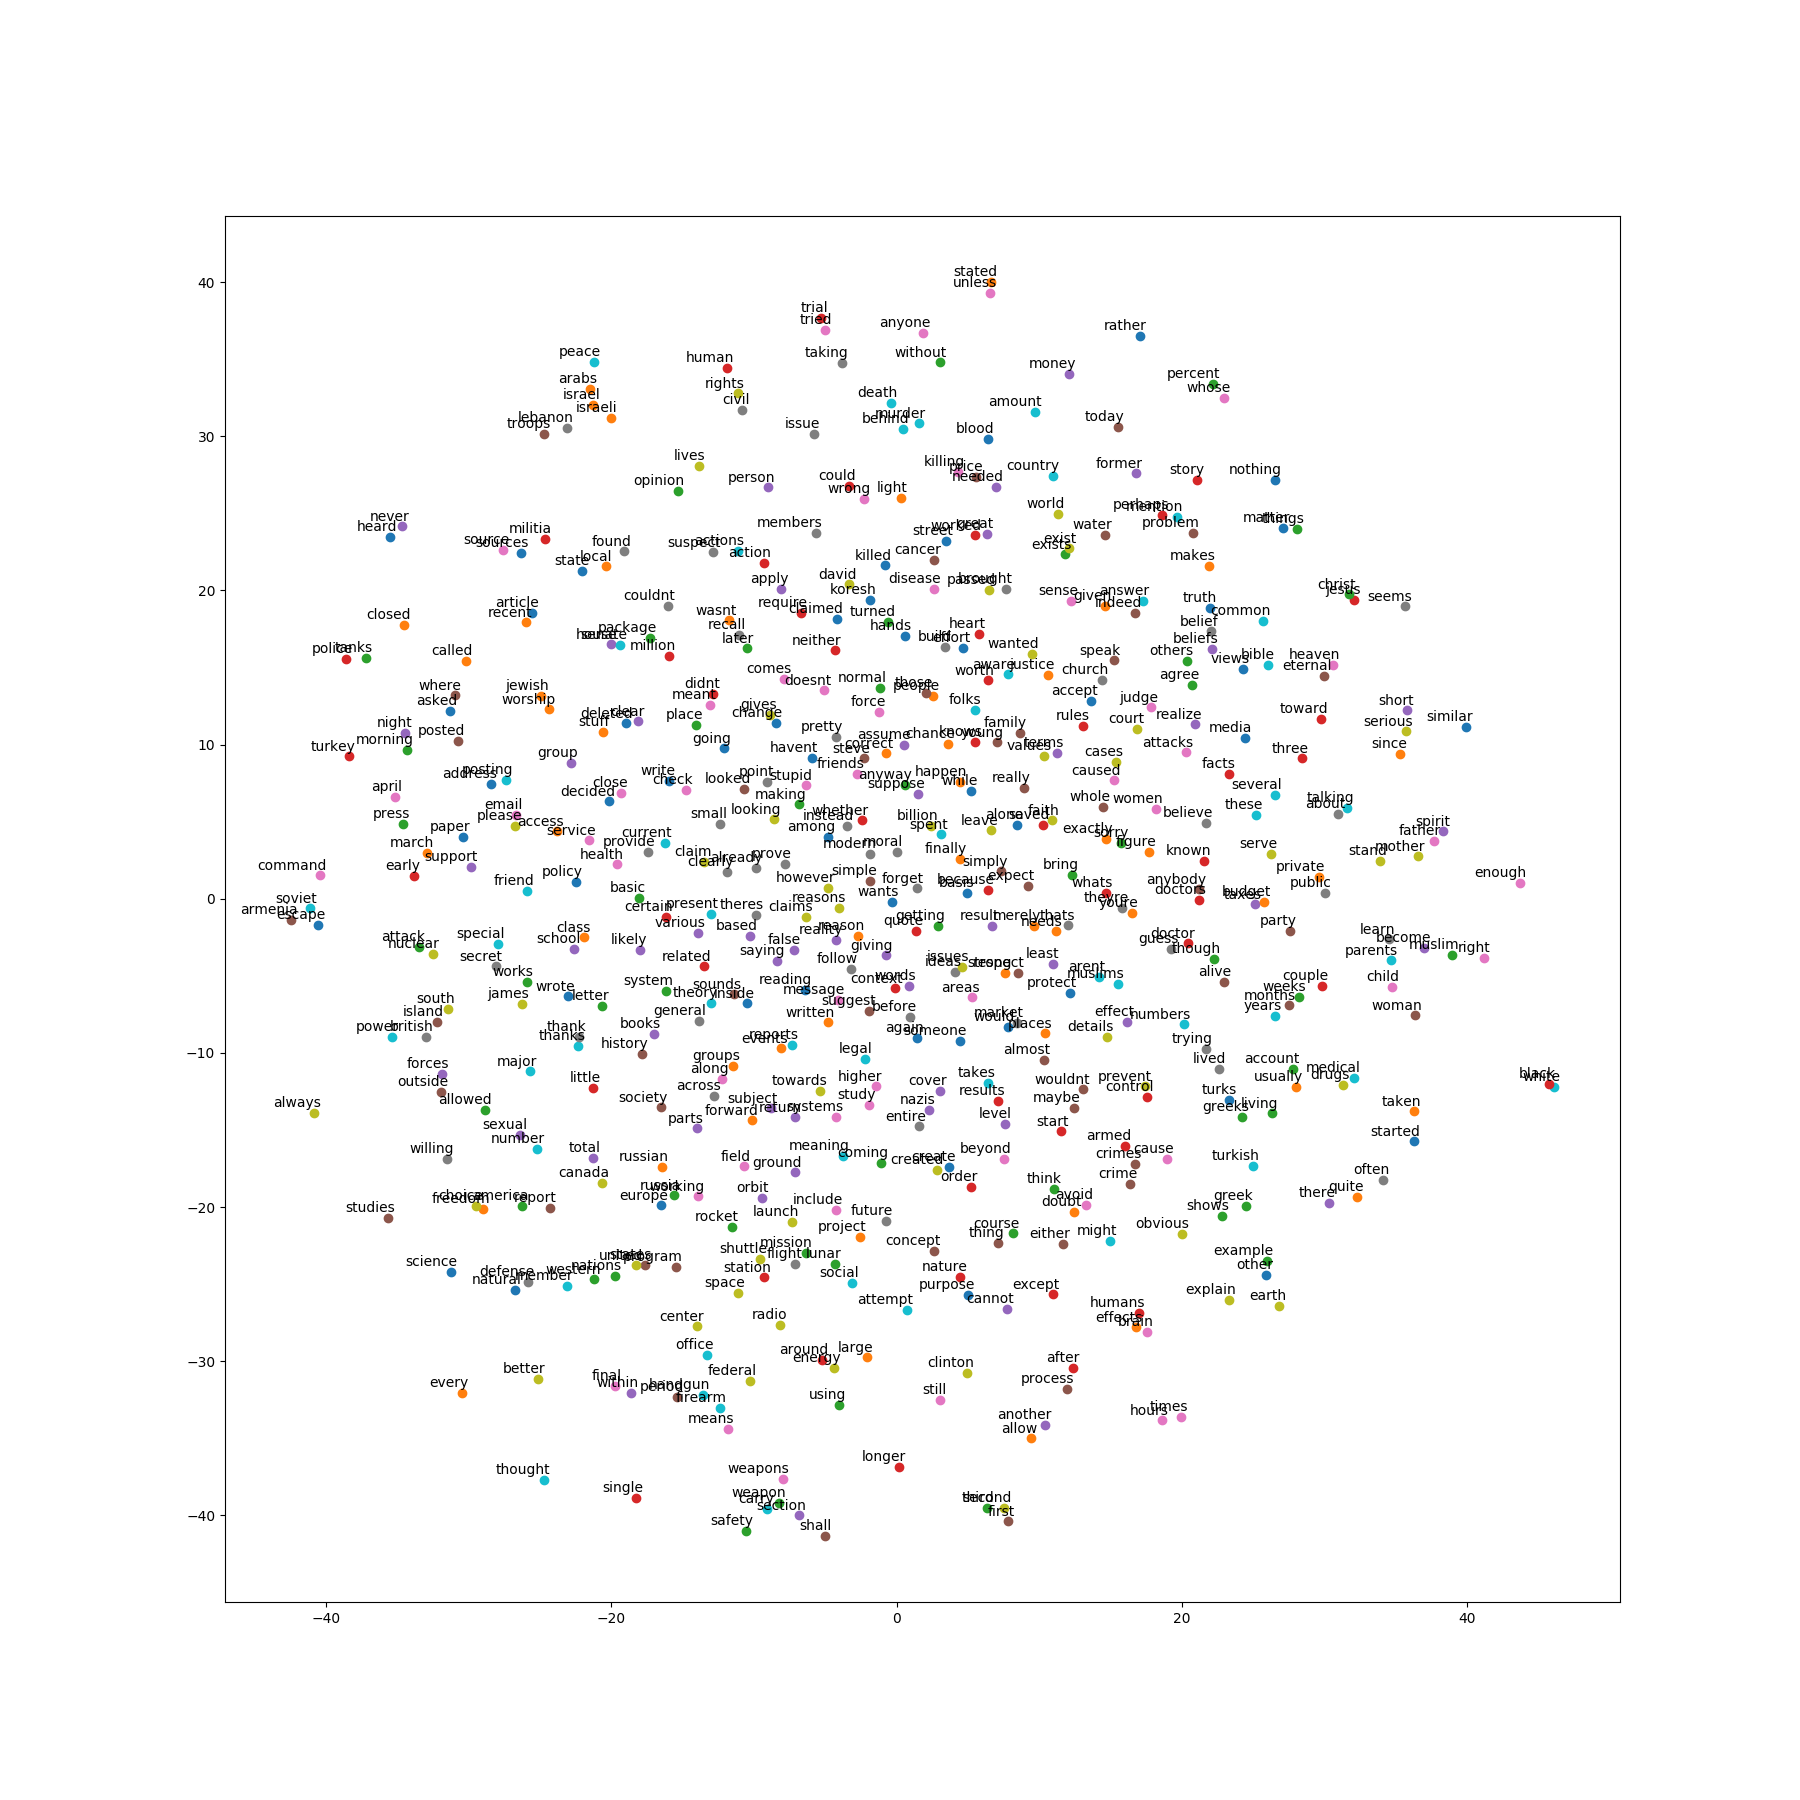
\includegraphics[width=18cm,height=15cm,keepaspectratio]{files/M128smallnews/M128smallnews.png}
  	\caption{t-SNE for KPCA skip gram model embeddings trained on vocabulary size of 20,000 words in 40,000 iteration on 20News dataset of size 350,000 words }
  	\label{fig:t1sne}
  \end{figure}
We also analyze the word embeddings using \texttt{k-nearest neighbors} of the words. These results in tables \ref{table:11} and \ref{table:13}, show that our model learns not only words with morphological similarity but also words with non-morphological similarity \textit{very quickly}.\\
In the table, \ref{table:11}, when we analyze the nearest neighbor of the word \texttt{"christ"}, at \texttt{step 0}, neighbors like \texttt{chris, christs} make sense. In the next iteration the model will start learning the semantically similar words also. At the \texttt{step 100,000} we have both semantic and morphological similar words as the nearest neighbors, \texttt{christs, savior, sinless, messiah}. Hence, initializing the model with KPCA embeddings helps the network to move towards the better neighbors "very fast".\\
 \begin{table}
 	\centering
\begin{tabular}{|l|l|l|}
	\hline
	\multicolumn{3}{|c|}{Skip gram Model with K-PCA Embeddings} \\
	\hline
	Step Number & Words & K=8 Nearest Neighbors of the word \\ \hline
	\multirow{2}{*}{Step 0} & \textbf{syria:} & wrong, wasps, hislop, falsely, randy, deacons, weary, japan \\
	& \textbf{christ:} & wrist, chris, christs, plink, sauna, opinons, cedar, mizrahi \\
	\hline
	\multirow{2}{*}{Step 20,000} & \textbf{syria:} & govt, syrian, basil, lumped, syrians, retain, holder, grossly \\
	& \textbf{christ:} & messiah, grace, lord, master, paul, christs, sins, savior \\
	 \hline
	\multirow{2}{*}{Step 40,000} & \textbf{syria:} & syrian, govt, jordan, israels, retain, syrians, dilemma, condone \\
	& \textbf{christ:} & christs, grace, messiah, savior, blessed, sins, praise, honor \\
	\hline
	\multirow{2}{*}{Step 80,000} & \textbf{syria:} & syrian, retain, jordan, israels, lebanon, sortees, sharp, govt \\
	& \textbf{christ:} & shalt, hast, christs, nutcase, savior, messiah, atoned, praise \\
	\hline
	\multirow{2}{*}{Step 100,000} & \textbf{syria:} &  syrian, retain, jordan, flows, sortees, lebanon, algeria, galilee\\
	& \textbf{christ:} & christs, shalt, savior, sinless, messiah, atoned, hast, nutcase\\
	\hline
\end{tabular}
\caption{The \textit{k}=8-nearest neighbors are generated for vectors of \textbf{128 dimension} on a vocabulary size of 20,000 words and dataset, \textbf{20NewsGroup} of size\textbf{350,000 words}}\label{table:11}
 \end{table}
%%TO DO longtable can be used 
We can also evaluate the vectors of different dimensions, \texttt{128 and 300} from tables \ref{table:11} and \ref{table:12}. Again the models are trained on same dataset and vocabulary. The vectors of dimension \texttt{300} are a bit better than those of \texttt{128}.
\begin{table}
	\centering
	\begin{tabular}{|l|l|l|}
	\hline
	\multicolumn{3}{|c|}{KPCA Skip gram Embeddings} \\
	\hline
	Step Number & Words & K=8 Nearest Neighbors of the word \\ \hline
	\multirow{2}{*}{Step 0} & \textbf{syria:} & syriac, myriad, syrias, myriads, syrian, tyrian, adrian, miriam \\
	& \textbf{christ:} & wrist, purist, christs, wrists, christi, purists, hristos, chris \\ 
	\hline
	\multirow{2}{*}{Step 20,000} & \textbf{syria:} & syrians, govt, syrian, jordan, itifada, soil, retain, viewed \\
	& \textbf{christ:} & lord, christs, depth, messiah, lucifer, gentile, bruise, creator \\
	\hline
	\multirow{2}{*}{Step 40,000} & \textbf{syria:} & syrian, jordan, retain, bombard, syrians, govt, sharp, itifada \\
	& \textbf{christ:} & messiah, honor, risen, savior, christs, sins, gentile, praying \\
	\hline
	\multirow{2}{*}{Step 80,000} & \textbf{syria:} & syrian, retain, jordan, lebanon, syrians, egypt, eldery, bombard \\
	& \textbf{christ:} & christs, savior, atoned, messiah, nutcase, velasco, againso, abraham \\
	\hline
	\multirow{2}{*}{Step 100,000} & \textbf{syria:} &  syrian, syrians, jordan, flows, sortees, lebanon, algeria, galilee\\
	& \textbf{christ:} & christs, messiah, savior, atoned, nutcase, againso, abraham, angel \\
	\hline
\end{tabular}
\caption{The \textit{k}=8-nearest neighbors are generated for vectors of \textbf{300 dimension} on a dataset, \textbf{20NewsGroup} of size, \textbf{350,000 words}}\label{table:12}
\end{table}
We can also evaluate the effect of data-set size from tables \ref{table:12} and \ref{table:13}. We can see that when trained on a larger dataset, our model tends to move more towards semantic similar vectors of the given word. It is also important to analyze that initializing the vectors with morphological similarity has given a huge boost to this move as in only 100,000 steps we have very nice semantic similar vectors which is not the case otherwise.
\begin{table}
	\centering
	\begin{tabular}{|l|l|l|}
		\hline
		\multicolumn{3}{|c|}{KPCA Skip gram Embeddings} \\
		\hline
		Step Number & Words & K=8 Nearest Neighbors of the word \\ \hline
		\multirow{2}{*}{Step 0} &\textbf{syria:} &syriac, myriad, syrias, myriads, syrian, tyrian, adrian, miriam\\
		& \textbf{christ:} &wrist, purist, christs, wrists, christi, purists, hristos, chris\\ 
		\hline
		\multirow{2}{*}{Step 20,000} & \textbf{syria:} &wily, dizzy, doorway, mayne, bald, keypad, subdued, frozen\\
		& \textbf{christ:} &burial, puts, rumors, heir, messiah, angel, truths, freely\\
		\hline
		\multirow{2}{*}{Step 40,000} & \textbf{syria:} &punjab, ciudad, sinai, libya, volga, spruce, surrey, aaai\\
		& \textbf{christ:} &lord, jesus, saints, birth, spirit, coptic, messiah, faith\\
		\hline
		\multirow{2}{*}{Step 80,000} & \textbf{syria:} &lebanon, serbia, annexed, latvia, jordan, peru, persia, turkey\\
		& \textbf{christ:} &saints, messiah, prophet, faith, mary, spirit, prayer, grail\\
		\hline
		\multirow{2}{*}{Step 100,000} & \textbf{syria:} &persia, israel, turkey, ukraine ,egypt, peru, lebanon, turkey\\
		& \textbf{christ:} &saints, messiah, prophet, baptism, mary, jesus, christian, spirit\\
		\hline
	\end{tabular}
	\caption{The \textit{k}=8-nearest neighbors are generated for vectors of \textbf{300 dimension} on a vocabulary size of 20,000 words and dataset, \textbf{Text8} of size,\textbf{17 million words}}\label{table:13}
\end{table}
When we evaluate our model word embeddings, trained for a morphological Language, \textbf{German}, we analyze that our model performs better than what it did for non-morphological language, \textbf{English}. Since most of the words which are morphologically similar, are also semantically similar, we can generate very similar neighbors in very few steps of training, as can be seen in table \ref{table:14}.
\begin{table}
	\hskip-1.5cm
	\begin{tabular}{|l|l|l|}
		\hline
		\multicolumn{3}{|c|}{KPCA Skip gram Embeddings} \\
		\hline
		Step Number & Words & K=8 Nearest Neighbors of the word \\ \hline
		\multirow{2}{*}{Step 0}
		& \textbf{macht:} &mitmacht, ohnmacht, aufmacht, ausmacht, machtlos, gemacht, lacht, gecoacht\\
		& \textbf{kinder:} &kinder-, rinder, inder, minder, binder, finder, linder, zylinder\\ 
		\hline
		\multirow{2}{*}{Step 20,000} 
		& \textbf{macht:} &aufmacht, achtung, gelacht, ansinnen, tatnacht, indische, nacht-, tafel\\
		& \textbf{kinder:} &eltern, familien, nachts, festtage, festem, festival, fests, festwirt\\ 
		\hline
		\multirow{2}{*}{Step 40,000} 
		& \textbf{macht:} &lacht, vielmehr, mache, anmelden, alltag, sorge, allemal, denke\\
		& \textbf{kinder:} &kindern, eltern, familien, lernen, gruppen, schule, betreut, lehrer\\ 
		\hline
		\multirow{2}{*}{Step 80,000} 
		& \textbf{macht:} &machte, mache, sorge, gemacht, versuche, sache, ehrgeiz, freude\\
		& \textbf{kinder:} &kindern, schueler, gruppen, lehrer, lernen, freunde, klassen, betreut\\ 
		\hline
		\multirow{2}{*}{Step 100,000} 
		& \textbf{macht:} &mache, machte, gemacht, hoert, sache, ehrgeiz, raeumt, merke\\
		& \textbf{kinder:}&kindern, gruppen, schueler, freunde, umgebung, lehrern, buechern, vereine\\ 
		\hline
	\end{tabular}
	\caption{The \textit{k}=8-nearest neighbors are generated for vectors of \textbf{300} dimension on a vocabulary size of 20000 words and subset of dataset, \textbf{news.2013.de}, of size, \textbf{52 million words}}\label{table:14}
\end{table}
We also evaluated the effect of increasing the vocabulary size as discussed in the section \ref{oov}. In table \ref{table:15}, we see that increasing the vocabulary size does not have a very major effect on the \textit{k}-nearest neighbors.
\begin{table}[H]
\begin{tabular}[htbp]{|l|l|l|l|}	
	\hline
	\multicolumn{4}{|c|}{\textbf{Comparing word2vec KPCA Embeddings with V=20,000 and V=118,000}} \\
	\hline
	\multirow{2}{*}{Step 100000}& \textbf{syria:}& sicily, ukraine, serbia, sudan& ukraine, persia, sudan, libya\\
	& \textbf{website:}& forum, site, archive, wiki &forum, site, archive, info, portal\\
	\hline
\end{tabular}
\caption{The \textit{k}=4-nearest neighbors are generated for vectors of \textbf{300} dimension on a vocabulary size of 20,000 words and vocabulary size of 118,000 words, on the dataset, \textbf{Text8}}
\label{table:15}
\end{table}

	\chapter{Evaluation}
\label{cha:eval}
In this chapter, we will evaluate our model with different parameters with the state of art model.
\section{Evaluating different Kernel PCA parameters}
From the figures, \ref{fig:k1} to \ref{fig:k4}, we can determine the appropriate kernel function that can be used for generating Kerneled PCA embeddings. In the figures, \ref{fig:k1} to \ref{fig:k4}, we computed different kernel functions on a set of words and then projected those kernel vectors on a 2-Dimensional space using Kernel PCA.
\begin{figure}[H]
	\begin{minipage}[b]{0.5\linewidth}
		\centering
		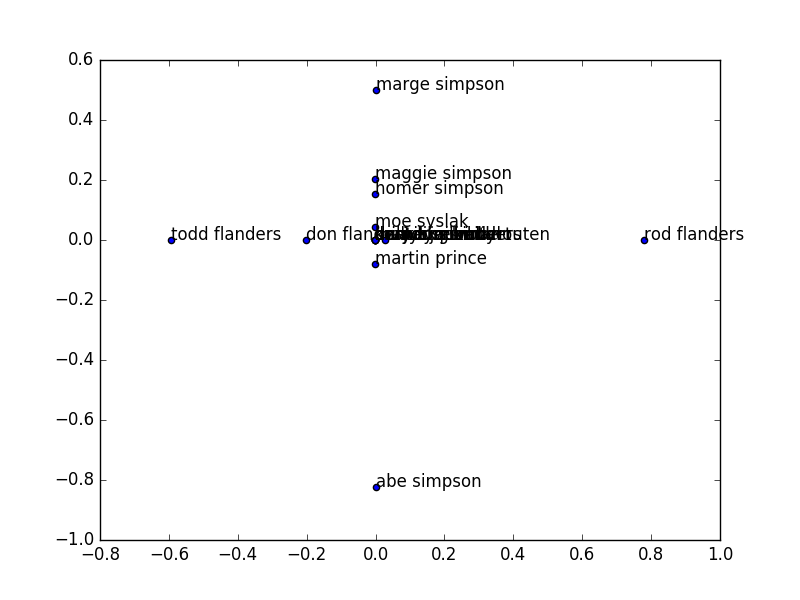
\includegraphics[width=1\linewidth]{files//KERNELPCA/log.png} 
		\caption{Logistic Kernel PCA} 
		\vspace{4ex}\label{fig:k1}
	\end{minipage}%%
	\begin{minipage}[b]{0.5\linewidth}
		\centering
		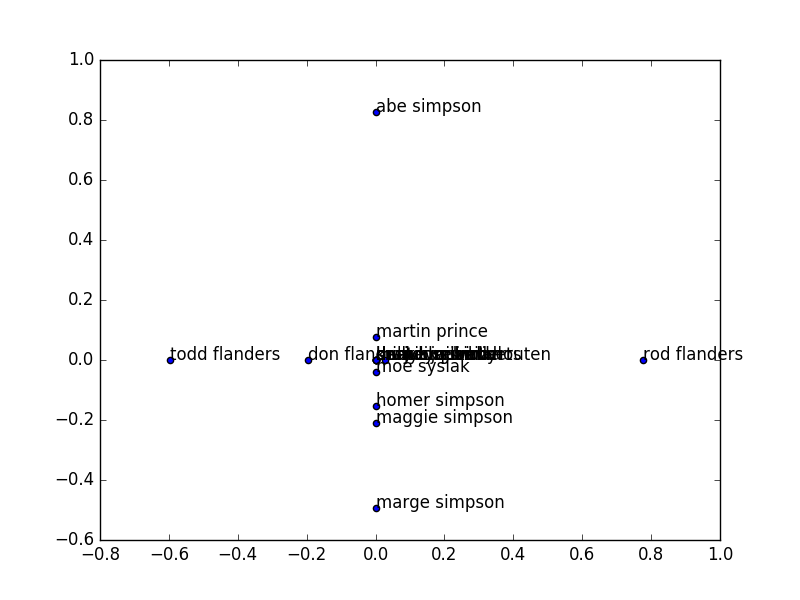
\includegraphics[width=1\linewidth]{files//KERNELPCA/cos.png} 
		\caption{Cosine Kernel PCA} 
		\vspace{4ex}\label{fig:k2}
	\end{minipage} 
\end{figure}
While the logistic and cosine kernel function does not work to cluster similar words together as seen in figures \ref{fig:k1} and \ref{fig:k2}, the polynomial and the Gaussian kernel works best in capturing the morphological similarity of words as demonstrated in figures, \ref{fig:k3} and \ref{fig:k4}. The Gaussian kernel is prominently used in such scenarios because it evaluates the kernel in an infinite dimensional space and hence is very flexible. The parameter sigma of the Gaussian kernel, which represents the co-variance, also plays a major role in its performance as it determine the width of the cluster, and hence should be carefully tuned according to the problem at hand.
\begin{figure}[H]
	\begin{minipage}[b]{0.5\linewidth}
		\centering
		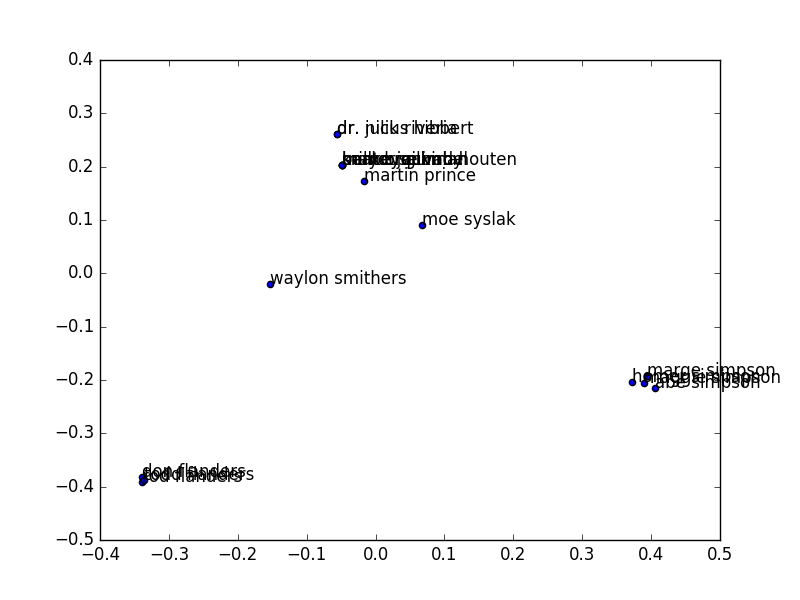
\includegraphics[width=1\linewidth,height=6cm]{files//KERNELPCA/gauss.png} 
		\caption{Gaussian Kernel PCA} 
		\vspace{4ex}\label{fig:k3}
	\end{minipage}%% 
	\begin{minipage}[b]{0.5\linewidth}
		\centering
		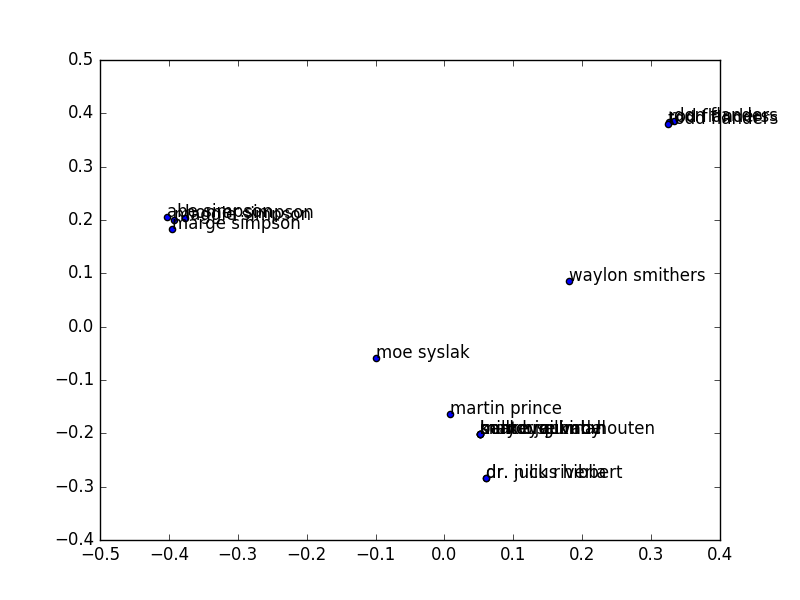
\includegraphics[width=1\linewidth]{files//KERNELPCA/poly.png} 
		\caption{Polynomial Kernel PCA(d=3)} 
		\vspace{4ex}\label{fig:k4}
	\end{minipage} 
	\label{fig:varKernel}
\end{figure}
\section{Evaluating Skip-gram Model trained using KPCA embeddings}
In this section, we will evaluate the performance of our KPCA skip gram model by comparing it against the performance of the basic skip gram model trained on the same parameters. Since the model follows an unsupervised approach, evaluation of the model can only be done using \texttt{"intrinsic evaluation tasks"}, which assess how well the vectors capture the word meaning and the relationships between those words. This is achieved using evaluating the models on the following tasks:
\begin{enumerate}
	\item \texttt{word similarity tasks}, that include finding a word's nearest neighbors.
	\item \texttt{word analogy tasks}, that include calculating the semantic and the syntactic similarity between the words.
\end{enumerate}
The \texttt{pre-trained Google embeddings}, which are considered to be the state of art embeddings, are trained on a dataset of size \texttt{100 Billion} words, with window size \texttt{5}, for \texttt{5} epoch using \texttt{12} threads running in parallel. One major challenge in the skip gram is that we have to train the model on a very large dataset to get the high quality vectors which creates problems, when we don't have a large dataset for training. The disadvantage of training a smaller dataset can  be eliminated by using our approach as we get fairly good quality word vectors, trained on a the relatively smaller dataset like \texttt{Text 8} and \texttt{20News Group} with only \textbf{"one epoch"}. The bad performance of basic skip-gram model in the following results, are  also been attributed to the fact that we are training the vectors on a these dataset. When we train the basic skip gram model on enWiki2016 dataset, as expected, the model starts doing well. 
\subsection{Word similarity Evaluation} 
One approach to evaluate the word embeddings is to see, how well they do in generating \textit{k}-nearest neighbors. This approach helps in visualizing the words and its most related neighbors. In tables \ref{x:1} and \ref{x_:2}, we compared the neighbors of the words, trained on both the models. When analyzed closely we find that our model starts to learn better word vectors rather quickly than the corresponding skip gram model in first few iterations. This is true for both the languages. In \texttt{German}, the results are even better because semantic similarity and morphological similarity converges. Hence fairly good results can be obtained even in fewer steps for morphologically rich languages. 
\begin{table}[H]
	\hskip-0.5cm
	\begin{tabular}[htbp]{|l|l|l|l|}	
		\hline
		\multicolumn{4}{|c|}{\textbf{Comparison between KPCA Skip gram Embeddings and basic Skip gram embeddings}} \\
		\hline
		Step Number&Word &K-PCA Embeddings & Word2vec Embeddings\\ \hline
		\multirow{2}{*}{Step 0} &\textbf{syria:}&syriac, myriad, syrias, myriads & czarist, driver, aurae, revert\\
		&\textbf{christ:}& wrist, purist, christs, wrists &robbing, backups, succeed, feud \\ 
		\hline
		\multirow{2}{*}{Step 20,000} & \textbf{syria:}&syrians, govt, syrian, jordan& czarist, driver, farid, revert \\
		& \textbf{christ:}&lord, christs, depth, messiah & succeed, robbing, axed, somalis \\
		\hline
		\multirow{2}{*}{Step 40,000} &\textbf{syria:}&syrian, jordan, retain, bombard& lebanon, kenneth, charlie, rocco\\
		& \textbf{christ:}&messiah, honor, risen, savior & somalis, succeed, squelch, axed\\
		\hline
		\multirow{2}{*}{Step 80,000} &\textbf{syria:}&syrian, retain, jordan, lebanon& lebanon, font, charlie, rocco\\
		& \textbf{christ:}&christs, savior, atoned, messiah & somalis, squelch, jesus, viscous\\
		\hline
		\multirow{2}{*}{Step 100,000} & \textbf{syria:}&syrian, syrians, jordan, flows& lebanon, font, charlie, rhode\\
		& \textbf{christ:}&christs, messiah, savior, atoned& somalis, squelch, jesus, viscous\\
		\hline
	\end{tabular}
	\caption{The \textit{k}=8-nearest neighbors are generated for vectors of \textbf{300} dimension on a dataset 20NewsGroup of size 17 Million words}\label{x:1}
\end{table}
With increased data set size, our model performed even better for generating the \textit{k}-nearest neighbors since it can learn better relationships by seeing more examples. This can be analyzed from the results in table, \ref{tabb:3}. 
But for the basic skip gram model, the performance is still bad since we are training a relatively smaller dataset with only 1 epoch. We have also demonstrated, in the same table, that our model works fairly well on all categories of words such as verbs, nouns, adjective etc.
\begin{table}[H]
	\hskip-2.0cm
	\begin{tabular}[htbp]{|l|l|l|l|}	
		\hline
		\multicolumn{4}{|c|}{\textbf{Comparison between KPCA Skip gram Embeddings and basic Skip gram embeddings}} \\
		\hline
		Step Number&Word &KPCA Skip gram Model & Skip gram Model\\ \hline
		\multirow{2}{*}{Step 0} &\textbf{macht:}&mitmacht, ohnmacht, aufmacht, ausmacht& witterete, haube, bereisen, skandle\\
		&\textbf{kinder:}&kinder-, rinder, inder, minder &chang,pflaume, schul-\\ 
		\hline
		\multirow{2}{*}{Step 20,000} & \textbf{macht:}&aufmacht, achtung, gelacht, ansinnen&zuercher, malte, naumburg, peitsche \\
		& \textbf{kinder:}&eltern, familien, nachts, festtage& hindurch, bedauert, jahrem winfried \\
		\hline
		\multirow{2}{*}{Step 40,000} &\textbf{macht:}&lacht, vielmehr, mache, anmelden& schon, zuercher, wurde, malte\\
		& \textbf{kinder:}&kindern, eltern, familien, lernen& jahre, schinm wurde, jahren\\
		\hline
		\multirow{2}{*}{Step 80,000} &\textbf{macht:}&machte, mache, sorge, gemacht& schon, immer, meuessen, jahren\\
		& \textbf{kinder:}&kindern, schueler, gruppen, lehrer& schon, jahre, jahren, immer\\
		\hline
		\multirow{2}{*}{Step 100,000} & \textbf{macht:}&mache, machte, gemacht, hoert& schon, immer, muessen, dabei \\
		& \textbf{kinder:}&kindern, gruppen, schueler, freunde& jahren, schon, viele, dabei \\
		\hline
	\end{tabular}
	\caption{The \textit{k}=8-nearest neighbors for vectors of \textbf{300} dimension generated from training the models on the subset of the dataset, \textbf{news.2013.de} of size 52 Million words for the morphological rich language: \textbf{German}} \label{x_:2}
\end{table}
\begin{table}
	\hskip-0.5cm
	\begin{tabular}[htbp]{|l|l|l|l|}	
		\hline
		\multicolumn{4}{|c|}{\textbf{Comparison between KPCA Skip gram Embeddings and basic Skip gram embeddings}} \\
		\hline
		Step No.&Word&K-PCA Embeddings& Word2vec Embeddings\\ \hline
		\multirow{6}{*}{Step 0}
		&\textbf{syria:}& syriac, myriad, syrias, syrian&inland, gally, shoham, myopic\\
		&\textbf{life:}& lmlife, lifes, wife, lift&dergisi, ream, alias, fifth\\
		&\textbf{india:}& indias, indigo2, indict, individ&wish, reuter, quills, ganja\\
		&\textbf{christ:}& wrist, purist, christs, wrists&july, citys, bushes, godism\\
		&\textbf{read:}& 5read, alread, ready, already&divided, masonry, haifa, capsule\\
		&\textbf{israeli:}& elihu, elijah, eliza, elize&rusty, spina, murphys, unites\\ 
		\hline
		\multirow{6}{*}{Step 20,000}
		&\textbf{syria:}& career, birth, your, beer&five, inland, four, zero\\
		&\textbf{life:}& reign, useful, atrophy, images&akita, alias, adder, nine\\
		&\textbf{india:}& induce, lady, vietnam, indulge&wish, three, from, nine\\
		&\textbf{christ:}& osiris, adopts, lips, phobia&july, with, univ, bushes\\
		&\textbf{read:}& survive, proven, involve, task&divided, masonry, haifa, capsule\\
		&\textbf{israeli:}& sylvia, jewry, paolo, elijah&rusty, akita, kansas, above\\ 
		\hline
		\multirow{6}{*}{Step 40,000} 
		&\textbf{syria:}& punjab, ciudad, sinai, libya&inland, five, four, whistle\\
		&\textbf{life:}& stages, career, spirit, faith&akita, zero, alias, adder\\
		&\textbf{india:}& vietnam, iran, berlin, mexico&wish, three, empires, colony\\
		&\textbf{christ:}& lord, jesus, saints, birth&july, bushes, escapes, rabies\\
		&\textbf{read:}& check, respond, tell, wait&divided, masonry, haifa, capsule\\
		&\textbf{israeli:}& serbian, wildly, tribal, weights&rusty, akita, kansas, above\\
		\hline
		\multirow{6}{*}{Step 80,000} 
		&\textbf{syria:}& lebanon, serbia, annexed, latvia&inland, whistle, peddle, judaic\\
		&\textbf{life:}& career, lives, stages, morning&akita, zero, adder, herod\\
		&\textbf{india}:& asian, baltic, brazil, vietnam&canada, africa, five, reuter\\
		&\textbf{christ:}& saints, messiah, prophet, faith&july, lied, citys, escapes\\
		&\textbf{read:}& learn, reader, hear, wants&divided, masonry, haifa, sided\\
		&\textbf{israeli:}& nato, iraqi, defence, inter&rusty, akita, zero, unites\\ 
		\hline
		\multirow{6}{*}{Step 100,000} 
		&\textbf{syria:}& persia, invaded, turkey, ukraine&inland, four, whistle, peddle\\
		&\textbf{life:}& lives, lifes, stages, shadow&akita, adder, zero, herod\\
		&\textbf{india:}& kuwait, vietnam, persia, turkey&thurs, canada, akita, seven\\
		&\textbf{christ:}& saints, messiah, prophet, baptism&july, lied, citys, bushes\\
		&\textbf{read:}& hear, check, learn, reader&haifa, divided, masonry, five\\
		&\textbf{israeli:}& iraqi, syrian, nato, libyan&rusty, akita, federal, murphys\\
		\hline
	\end{tabular}
	\caption{The \textit{k}=8-nearest neighbors are generated for vectors of 300 dimension on a dataset size of \textbf{17 million words}}\label{tabb:3}
\end{table}

We can also visualize, how well our model did by plotting the t-SNE embeddings of a subset of words from the dictionary.
In this evaluation, we have used \texttt{t-SNE} to project word embeddings on a 2 dimensional space to get a better visualization of the similar word vectors. We obtained visualization of these t-SNE plots for embeddings trained on different datasets and vocabulary sizes, plotted in figures \ref{fig:tsnee1} to \ref{fig:tsnee5}. As expected, we can see that the words which have high similarity are clustered. On comparing t-SNE of our approach with that of skip gram model, we can very easily say that similar words clusters are more prominent in our approach. 

On further analysis of these plots, we can say that even when we add more words to our small vocabulary fig. \ref{fig:tsnee3}, its performance is very much comparable to the fig. \ref{fig:tsnee2}. This proves that we can increase our vocabulary easily with \textbf{Out-Of-Vocabulary words} using method explained in the section \ref{oov}, before training the skip gram model with KPCA embeddings. We also analyzed that there is not a prominent drop in performance of our model when a large number of words are added. It still performs better than the corresponding skip-gram model as seen in figure, \ref{fig:tsnee1}. \\
We also saw the effect of data set size on the basic skip gram performance in figures, \ref{fig:tsnee1} and \ref{fig:tsnee5}. After analyzing these t-SNE plots, we can confidently say that the skip gram model's performance for clustering the similar words starts improving, when it is trained on a bigger dataset. In figure, \ref{fig:tsnee5}, since the dataset is of size 52 million words, we can trace some clusters.
\begin{figure}[H]
	\hskip-2cm
	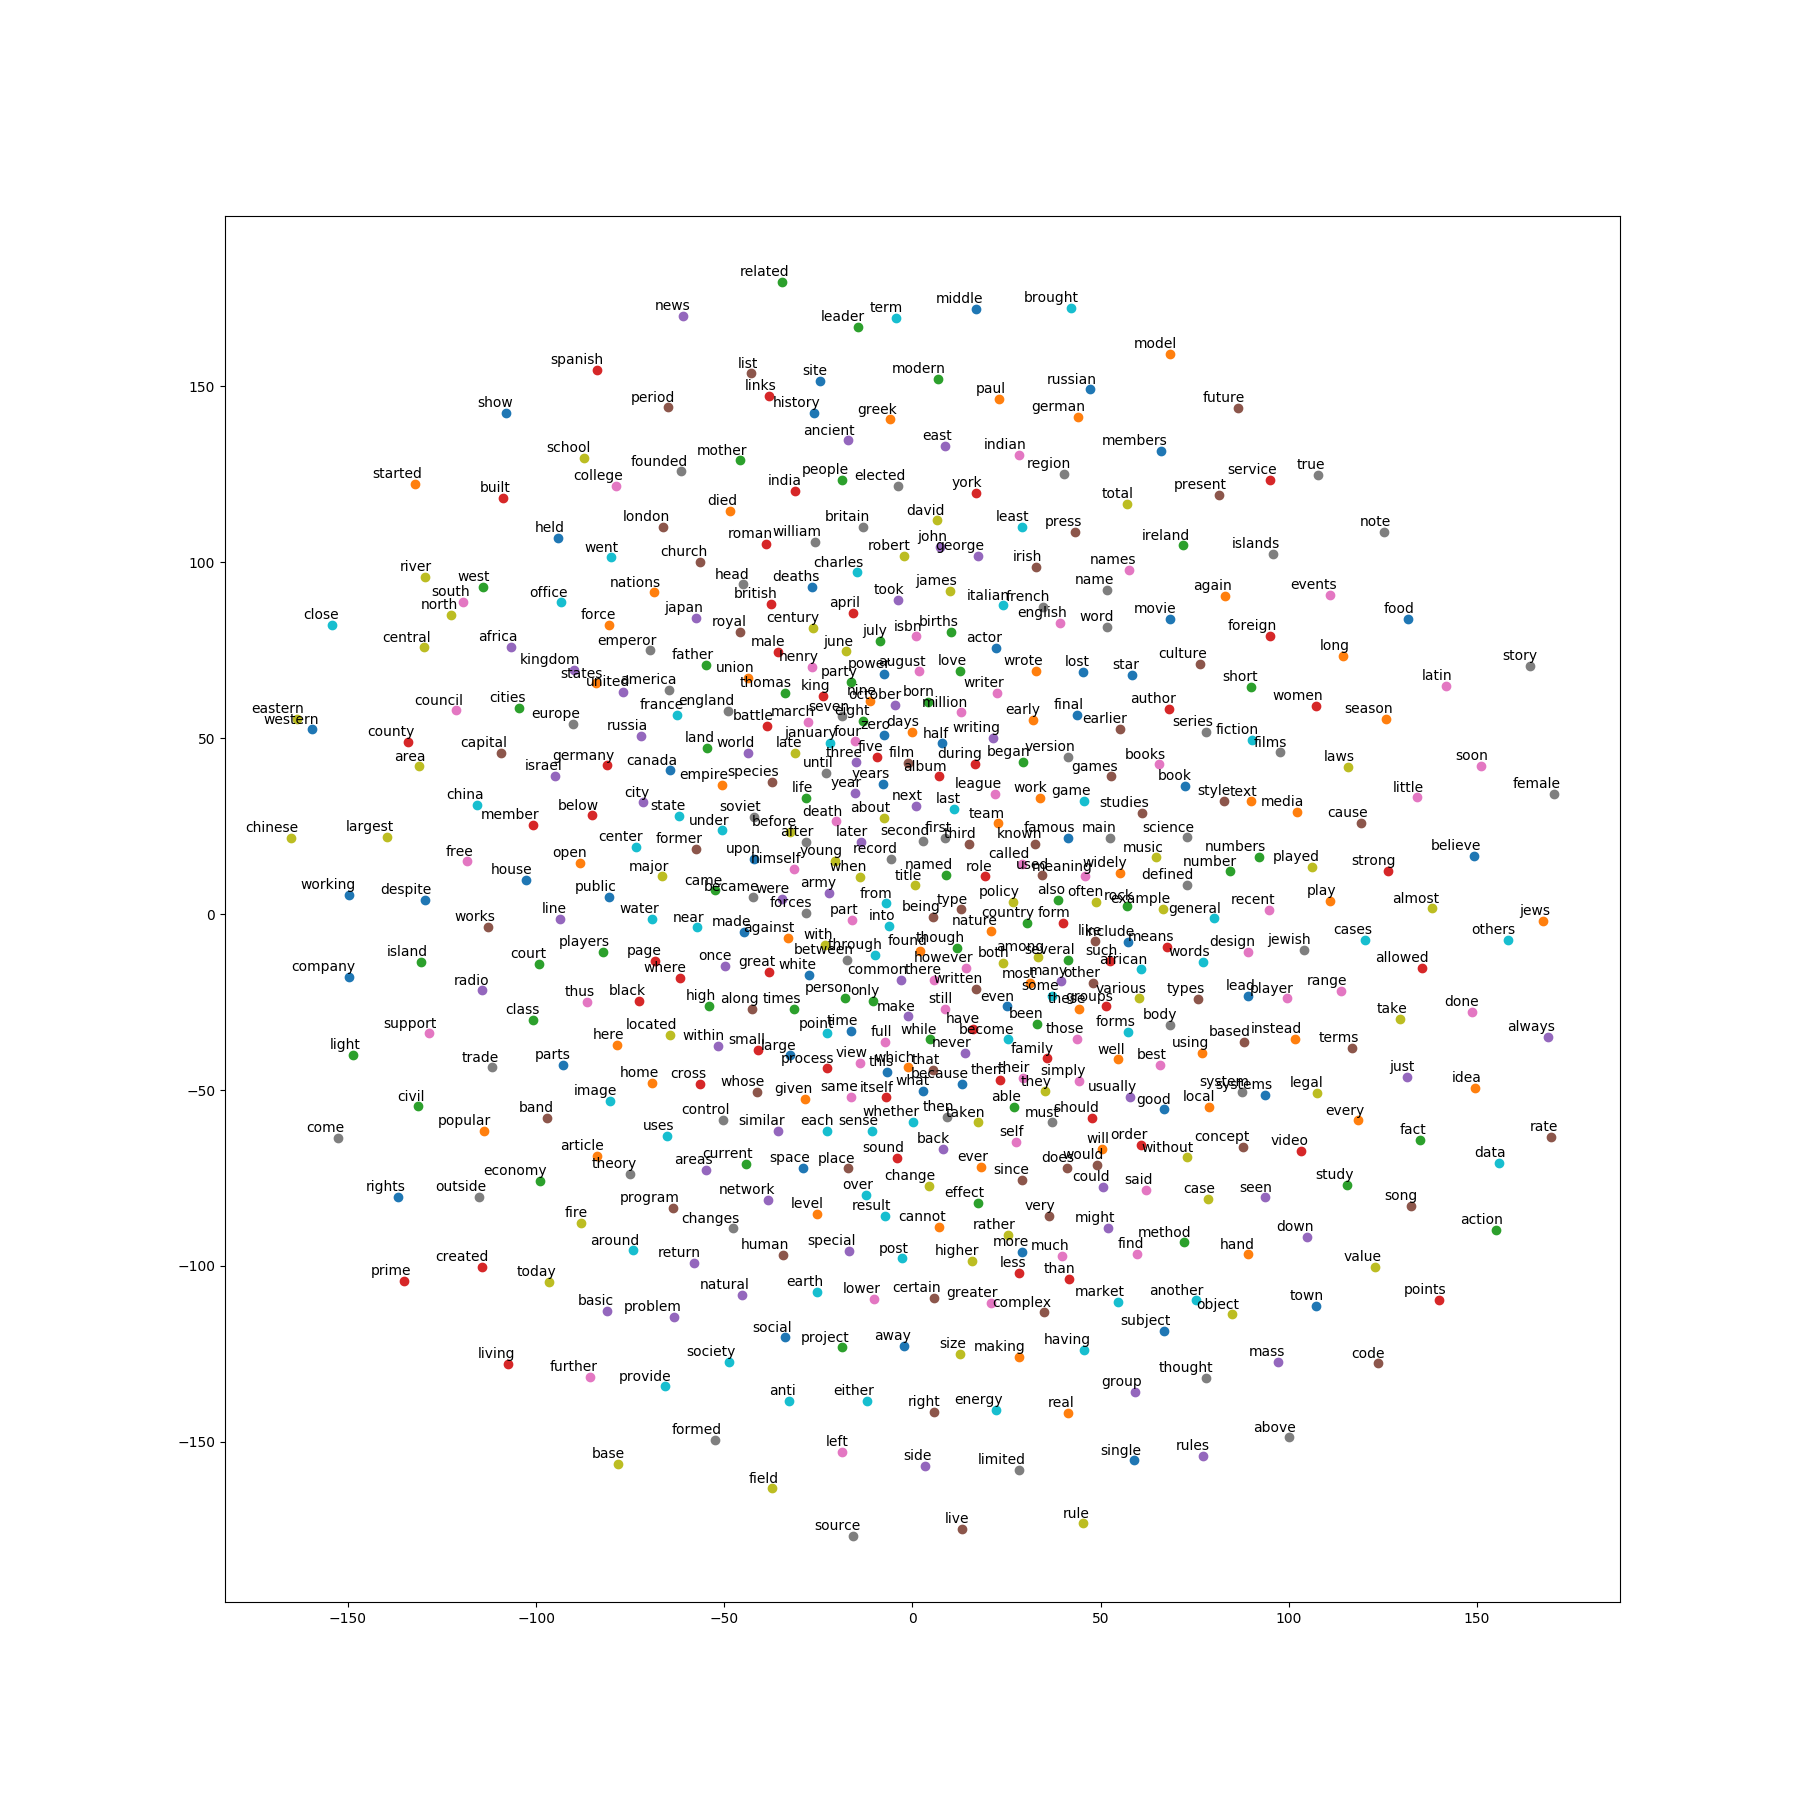
\includegraphics[width=20cm,height=20cm,keepaspectratio]{files/enText8-20kExtendedVocab/w2vtsne.png}
	\caption{t-SNE visualization of Skip gram model with vocabulary size 118,000 trained in 100,000 iteration on Text8 dataset. On analyzing this plot, we cannot find any prominent cluster. The bad performance of the model can be attributed to the fact that we are training the model on a relatively smaller database for 1 Epoch. The performance ought to improve when we train the model for more epoch which is illustrated in later section, in table,\ref{tab:sesx}}
	\label{fig:tsnee1}
\end{figure}
\begin{figure}[H]
	\hskip-2cm
	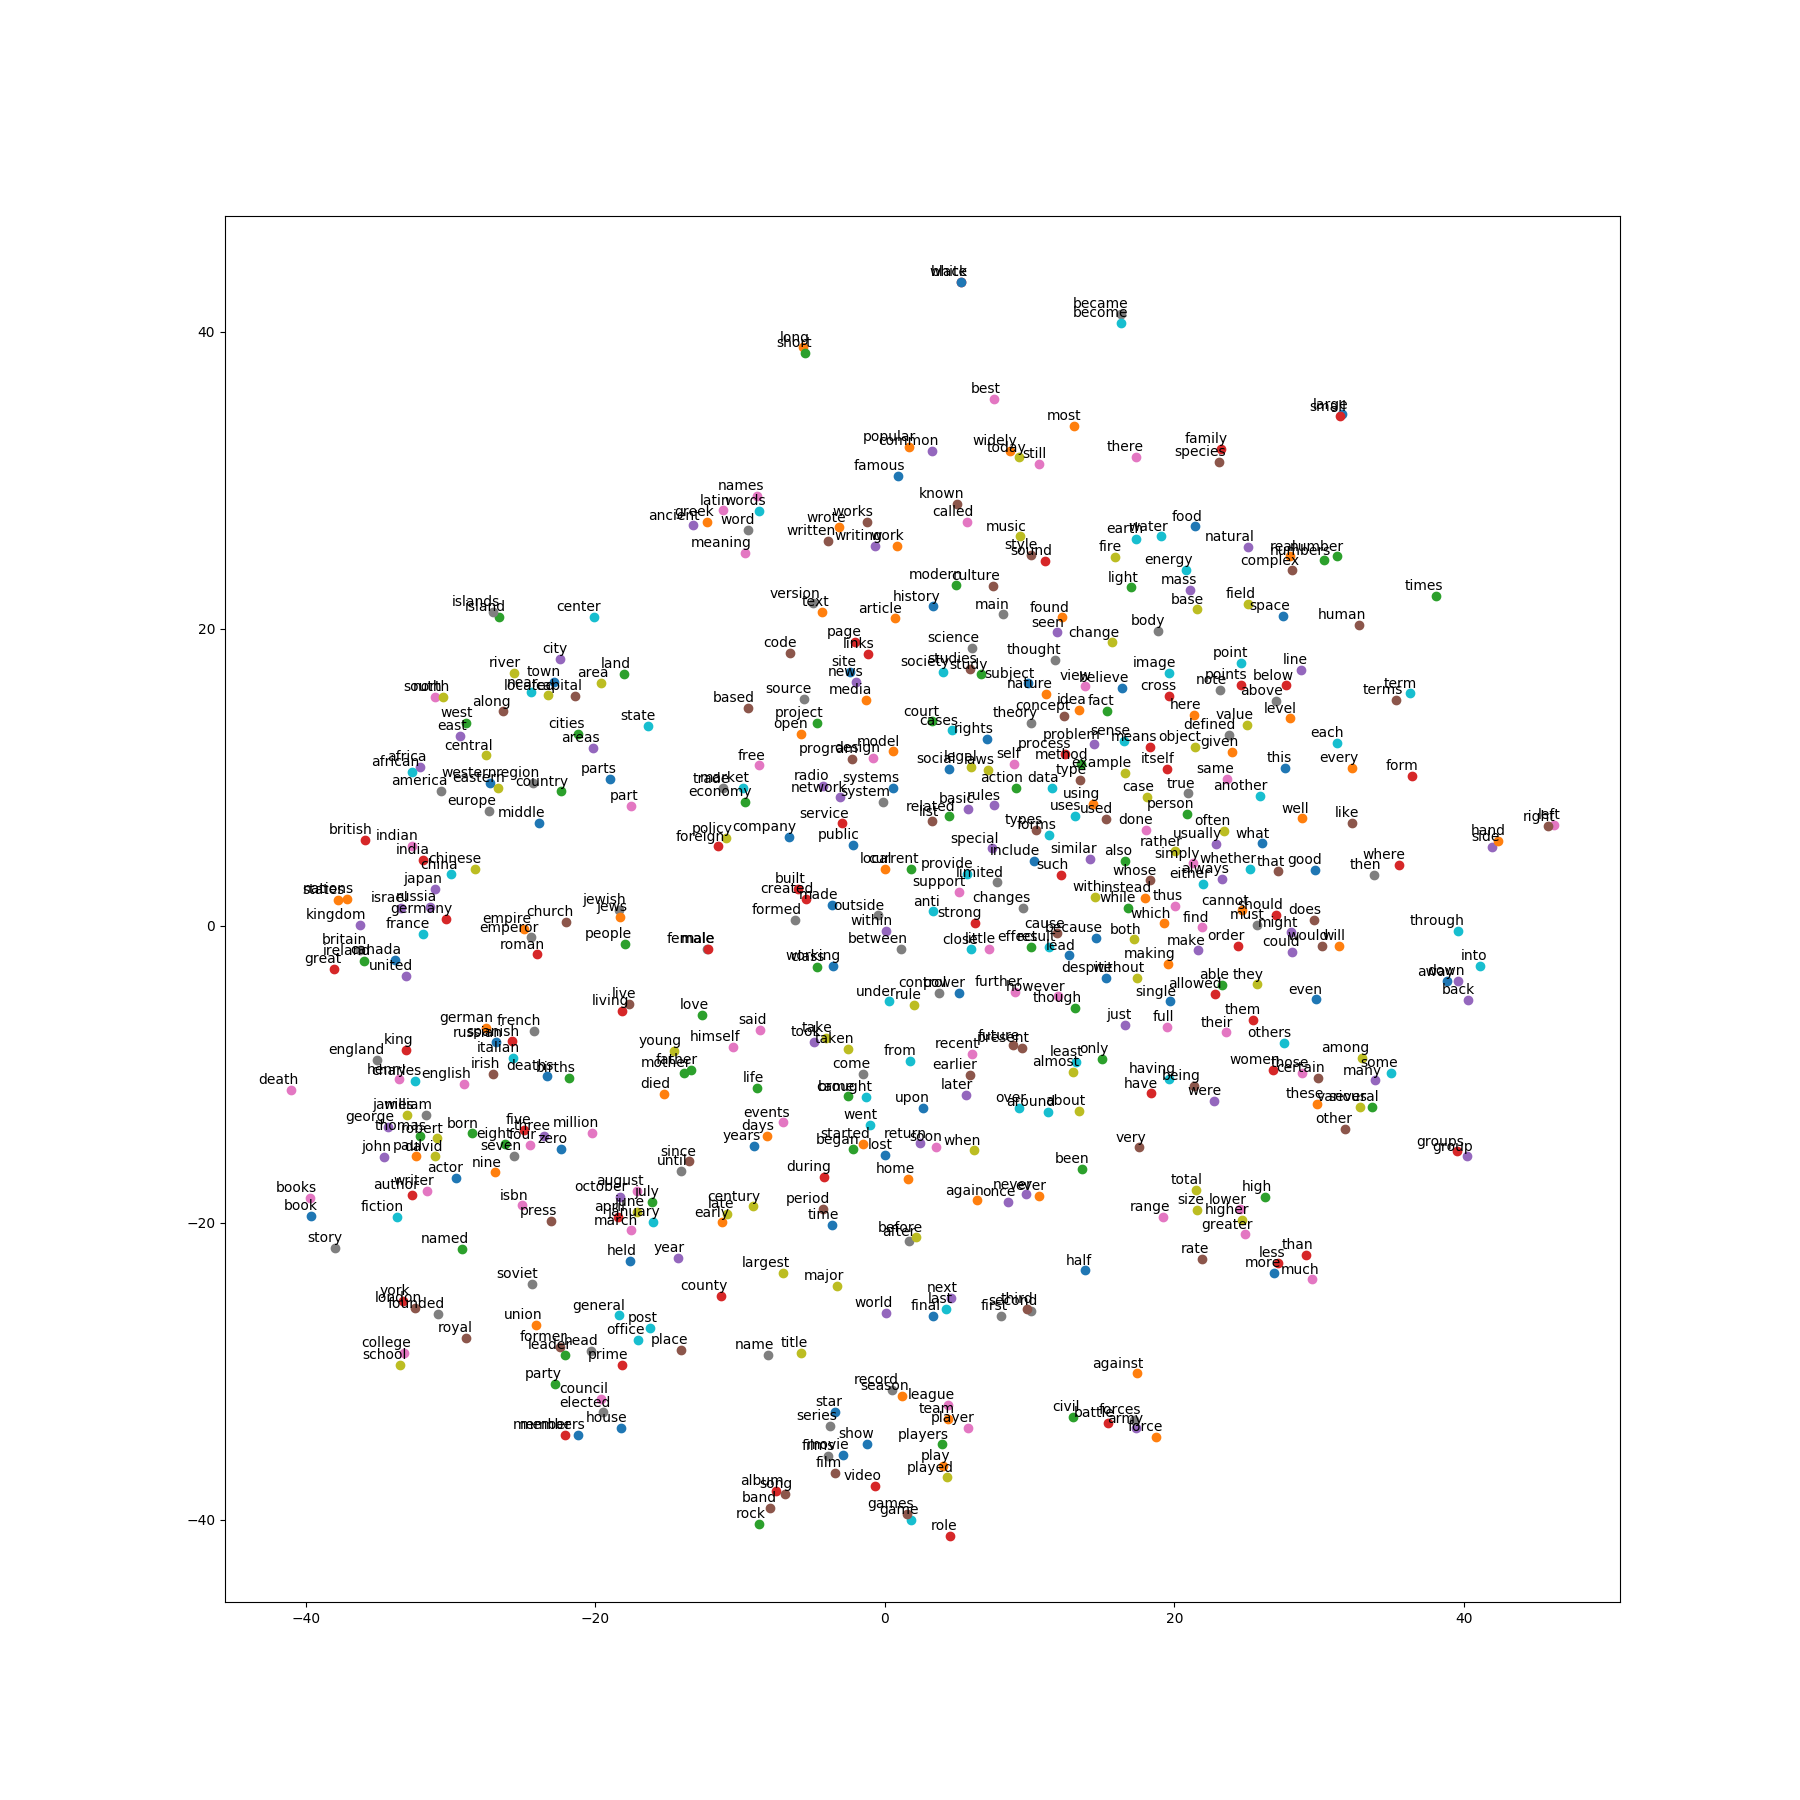
\includegraphics[width=20cm,height=20cm,keepaspectratio]{files/enText8-20kExtendedVocab/text8V20000.png}
	\caption{t-SNE visualization of KPCA Skip gram Word embeddings for vocabulary size 20,000, trained in 100,000 iterations on Text8 dataset of size 17 Million words. If analyzed closely, we find all the nations are clustered together. First names, natural areas, hobbies types and degree of comparison also form very prominent clusters.}
	\label{fig:tsnee2}
\end{figure}
\begin{figure}[H]
	\hskip-2cm
	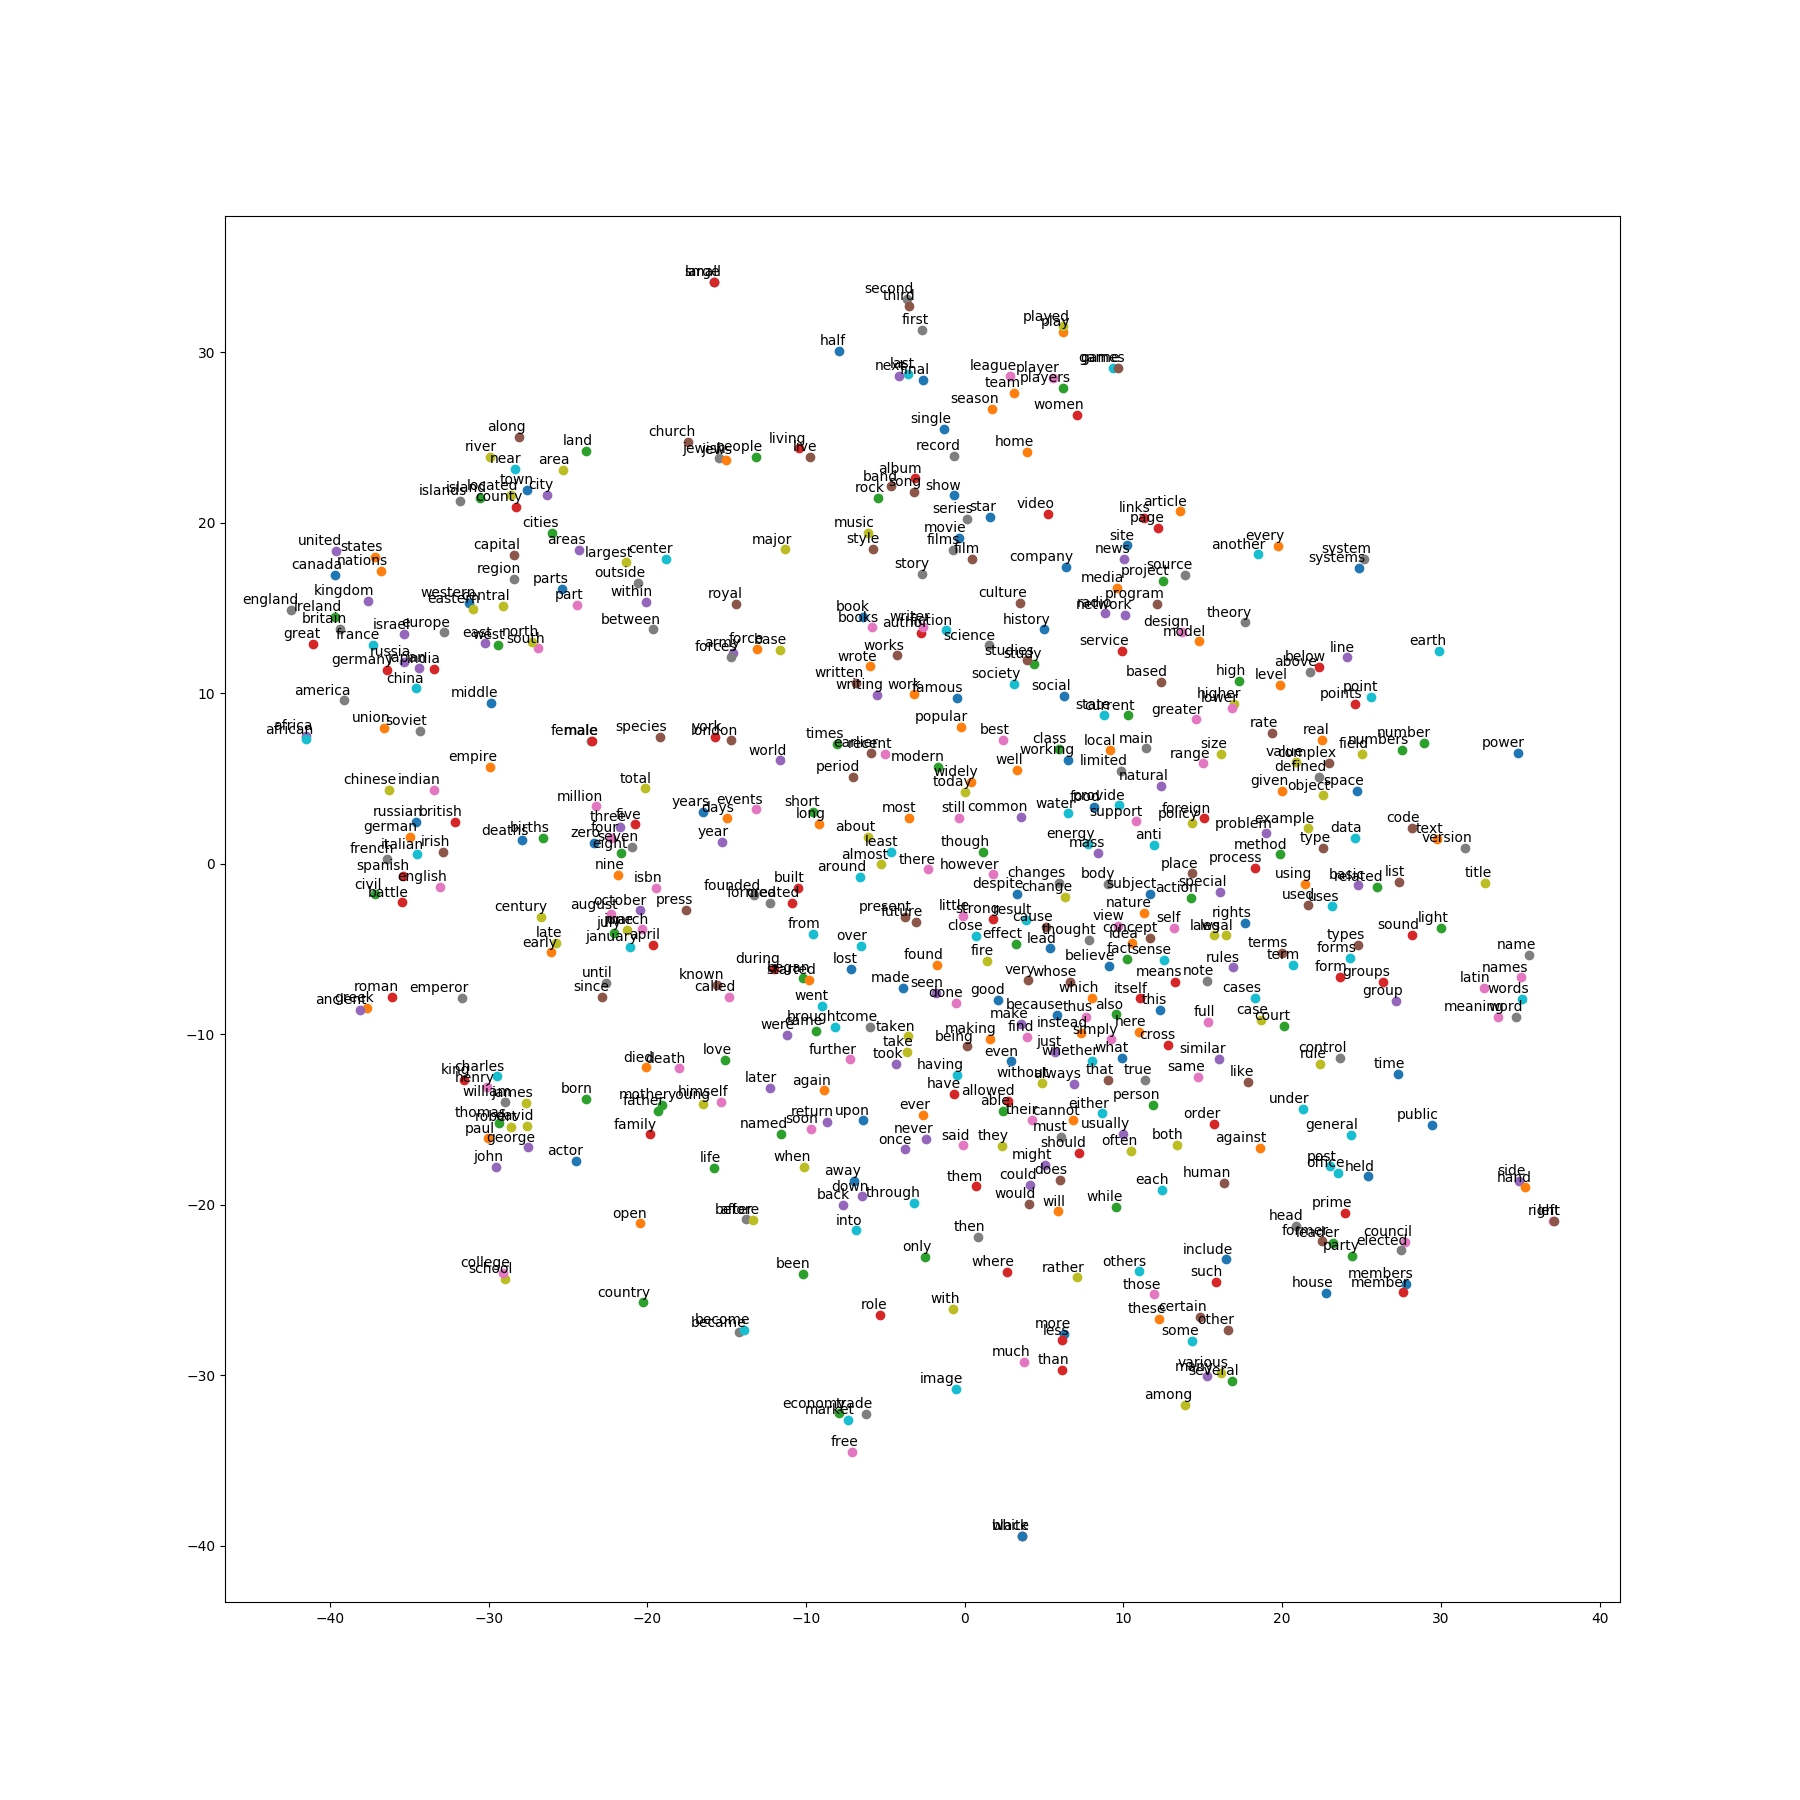
\includegraphics[width=20cm,height=20cm,keepaspectratio]{files/enText8-20kExtendedVocab/tsne.png}
	\caption{t-SNE visualization of KPCA Skip gram embeddings with Vocabulary size 20,000 words extended to 118,000 words, trained in 100,000 iteration on Text8 dataset of size 17 Million words. If analyzed closely, we find clusters of nationality, nations, first names etc. Another important thing to note is that clusters of the nationality and the nations also lie close to each other. }
	\label{fig:tsnee3}
\end{figure}

\begin{figure}[H]
	\hskip-2cm
	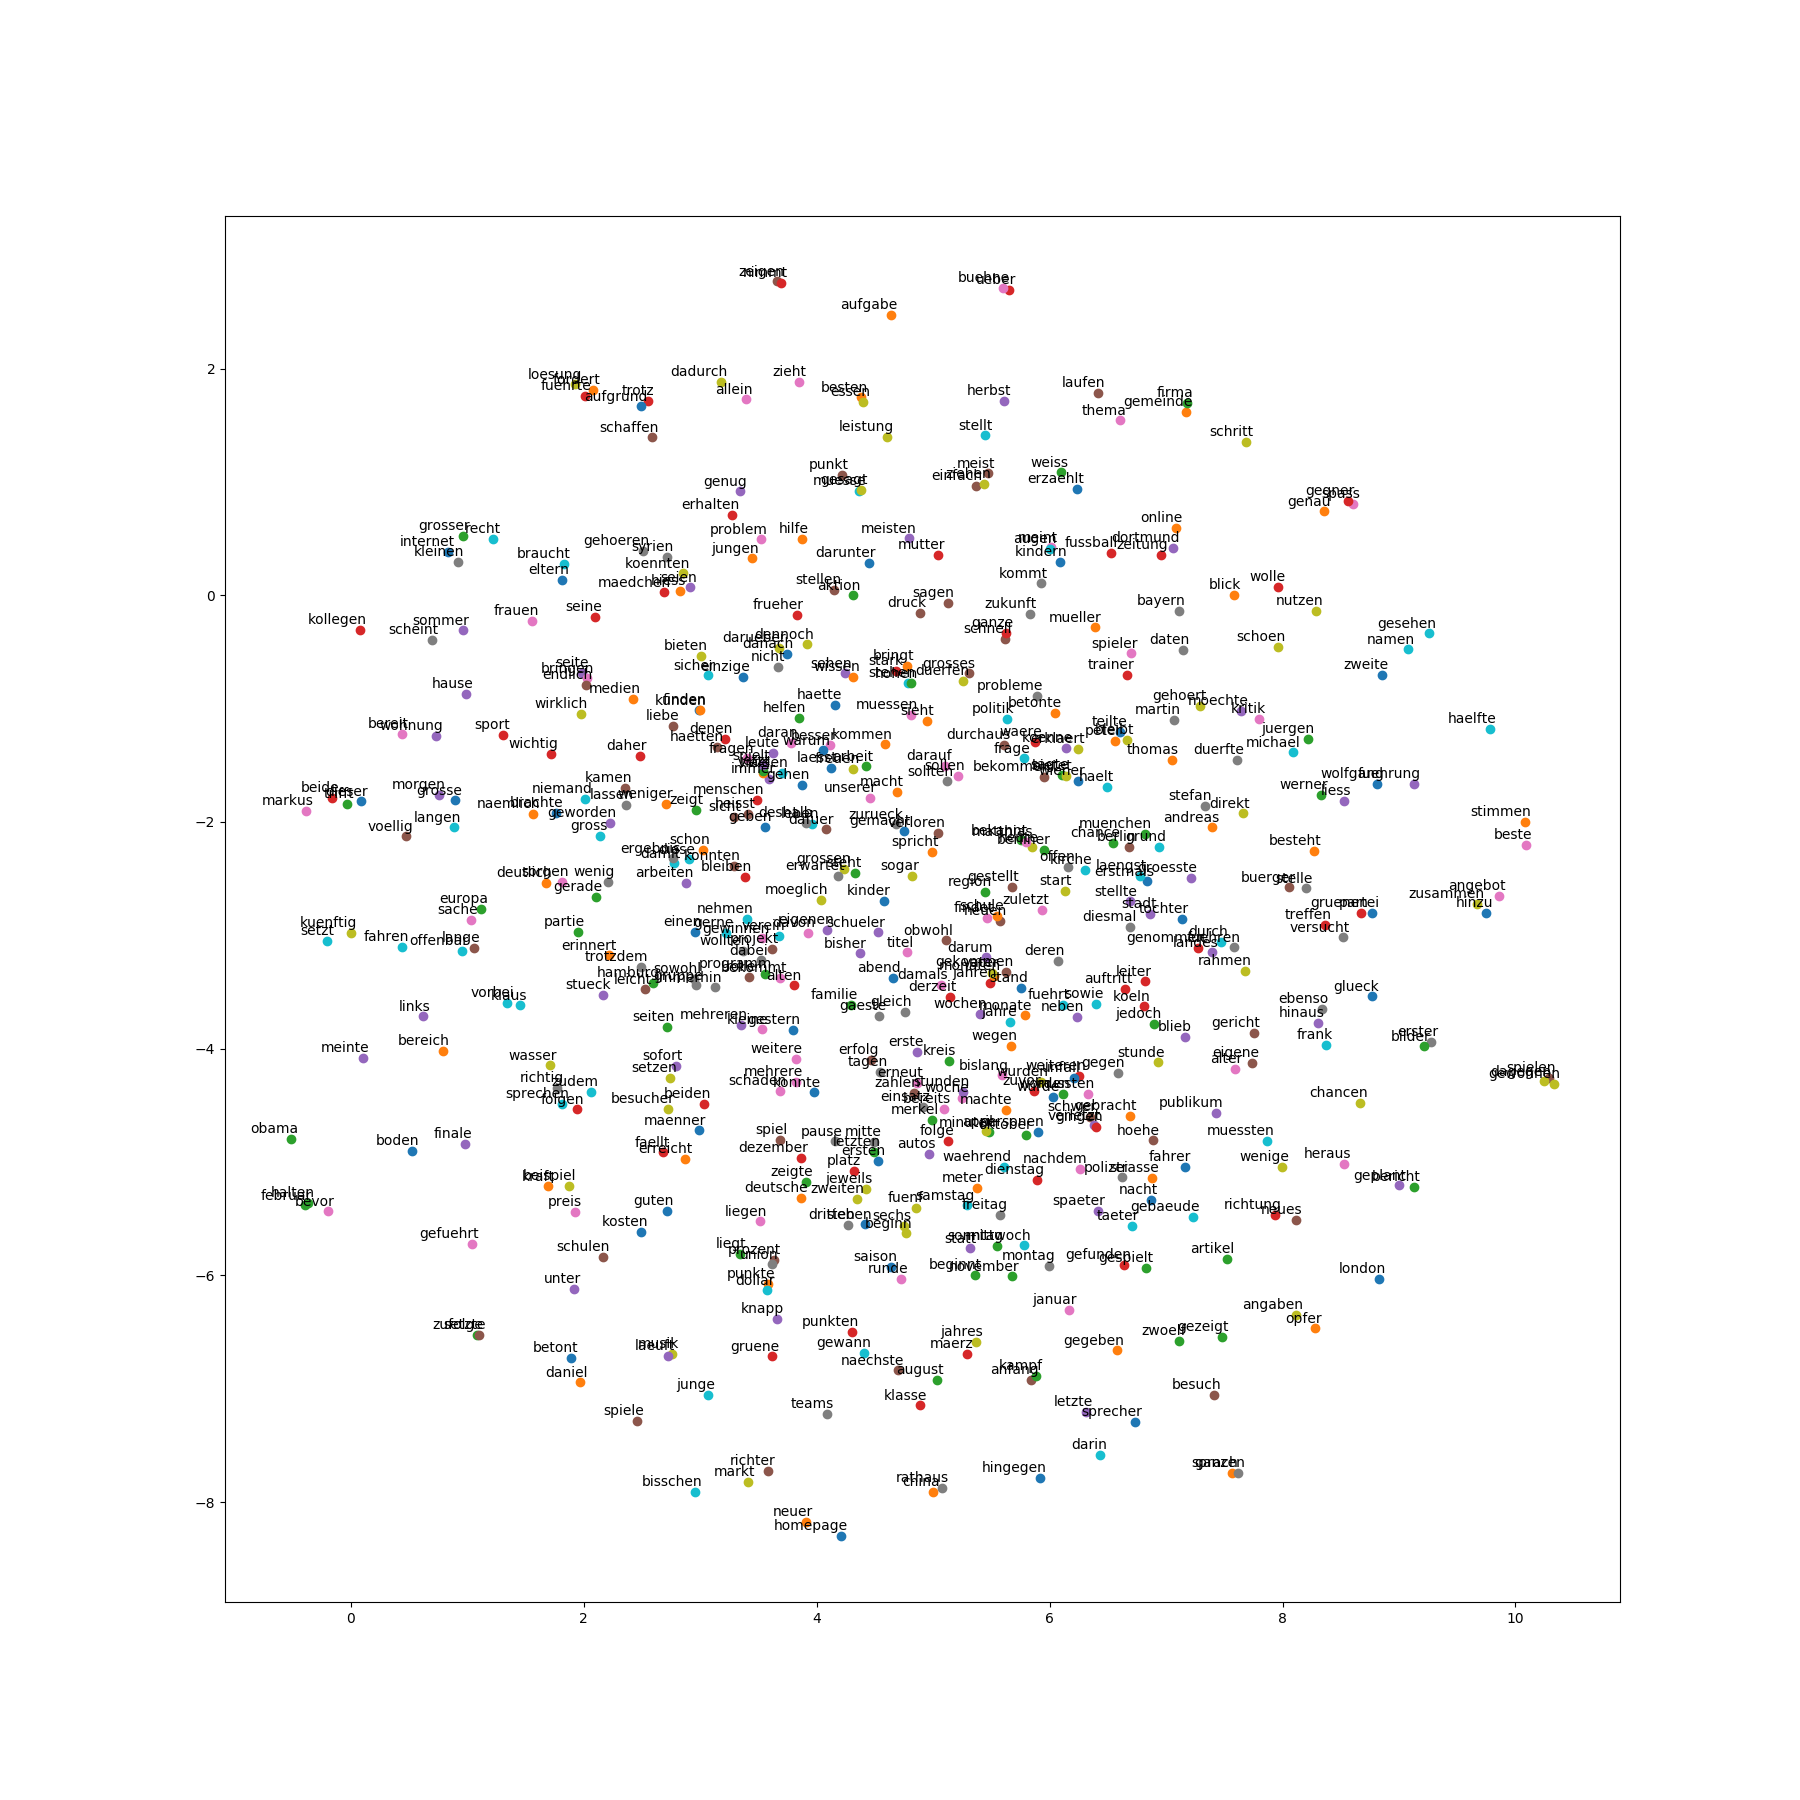
\includegraphics[width=20cm,height=20cm,keepaspectratio]{files/deWiki20kVocab/tsne.png}
	\caption{t-SNE visualization of Skip gram model with Vocabulary size 20,000 trained in 100,000 iteration on a subset of dataset news.2013.de.shuffled.corpus of size 52 Million words. When analyzed closely, we find verbs such as "nehmen", "arbeiten", "bleiben" got clustered together. Other example is words like "mehreren", "mehrere", "weiter" also got clustered}
	\label{fig:tsnee4}
\end{figure}
\begin{figure}[H]
	\hskip-2cm
	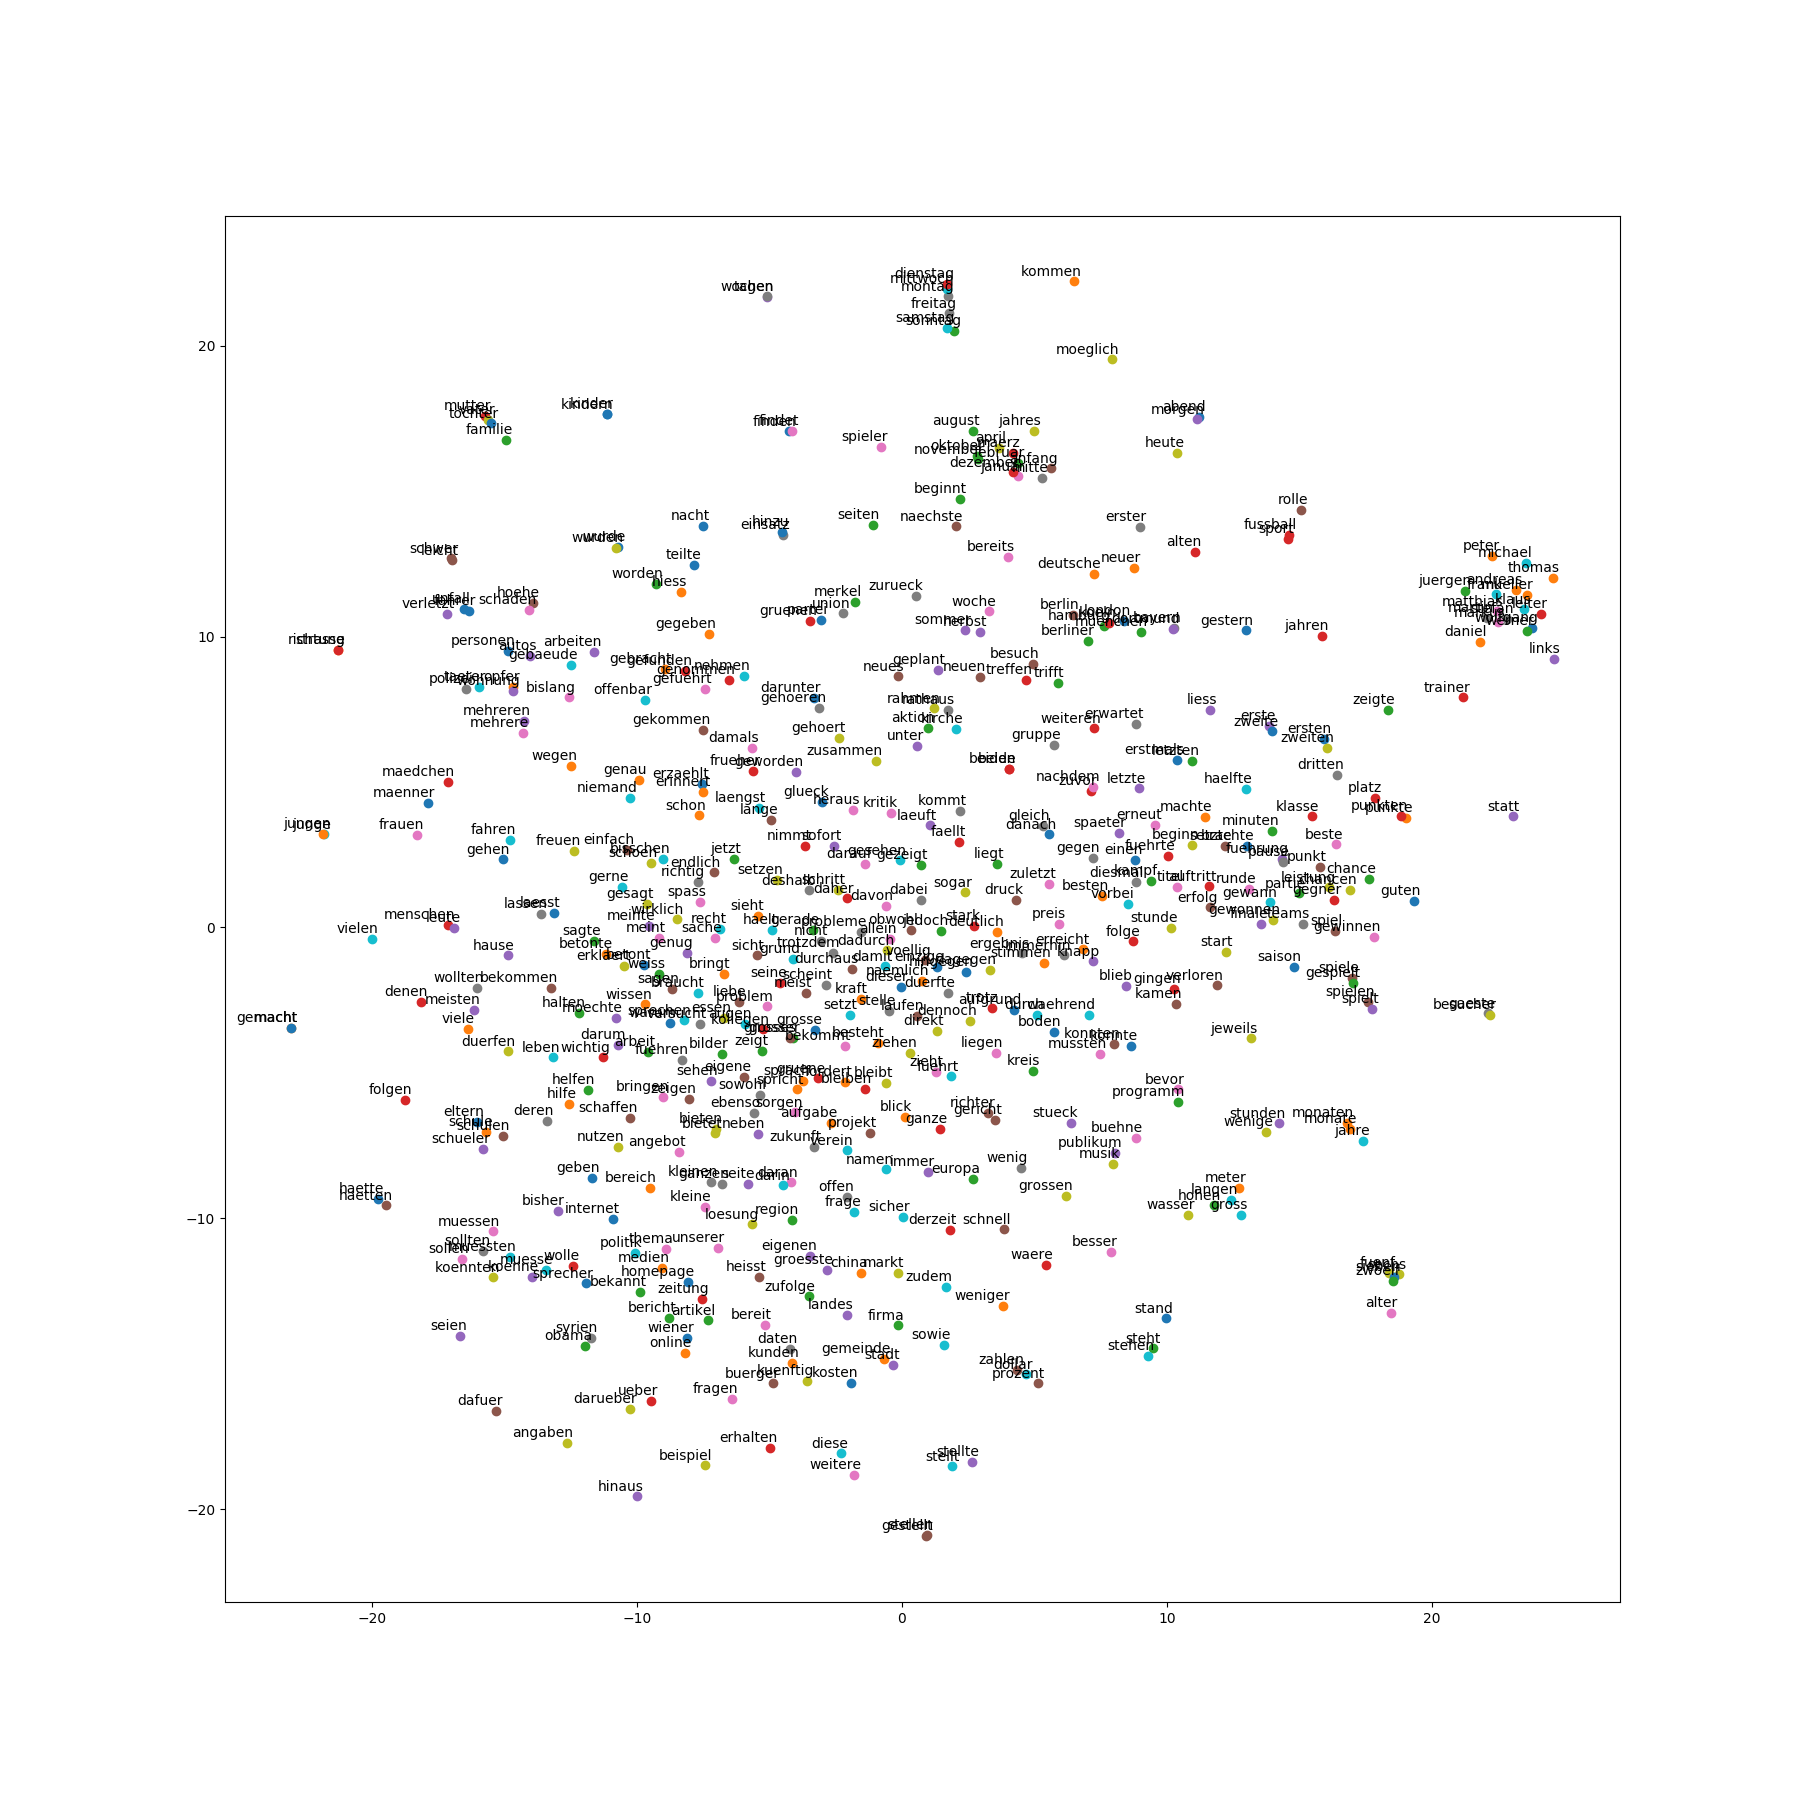
\includegraphics[width=20cm,height=20cm,keepaspectratio]{files/deWiki20kVocab/MYtsne.png}
	\caption{t-SNE visualization of KPCA Skip gram embeddings with vocabulary size 20,000 trained in 100,000 iteration on a subset of dataset news.2013.de.shuffled.corpus of size 52 Million words. When analyzed closely, we find prominent clusters of weekday names, first names, family memeber types etc.}
	\label{fig:tsnee5}
\end{figure}
 
To summarize word similarity evaluation, we can say that KPCA Skip gram Model performs far better than the basic skip gram model. This can be attributed to the fact that we already have trained the vectors for morphological similarities. The model just needs to learn the semantic and syntactic similarity. Since basic skip gram model learns morphological similarity implicitly so initializing the model with those helps in speed up the process of convergence. The performance is even better when the language is rich in morphemes such as German.
%% german k nearest neighbors for 300 dim
\subsection{Word Analogy Evaluation}
In their paper, \cite{mikolov2013efficient} stated that when we train the high dimensional word vectors on a very large data set, the vectors also learn very subtle relation between the words, for example relationships between the country and its capital city.  The figure, \ref{fig:t3}, from paper \cite{mikolov2013distributed}, demonstrates such a relationship. 
\begin{figure}[H]
	\centering
	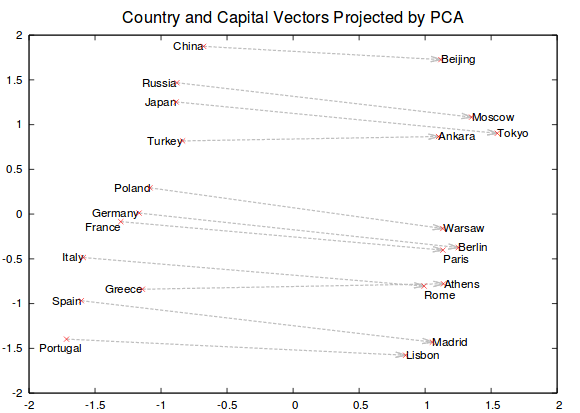
\includegraphics[width=10cm,height=8cm,keepaspectratio]{files/3.png}
	\caption{ Two-dimensional PCA projection of the \textbf{1000-dimensional} Skip-gram vectors of countries and their capital cities as demonstrated by \cite{mikolov2013distributed}}
	\label{fig:t3}
\end{figure}
The data set used to obtain these state of art results, was of 6 Billion words in size and vector dimensions produced were of 1000 dim. In this comparison, our model learned these relationship quickly  we already have morphological similarities encoded in the input vectors. Thus we do not need a large amount of data to train our model. This is very well demonstrated in the figures \ref{fig:t} and \ref{fig:d} where we have plotted the country and the capital relationships for both the models (in both the languages). From these plot we can state that our model has learned these similarity not only in fewer steps but also in a lower dimensional space when compared to the basic skip gram trained using the same parameters. 
\begin{figure}[htbp]
	\centering
	\subfloat[KPCA skip gram model]{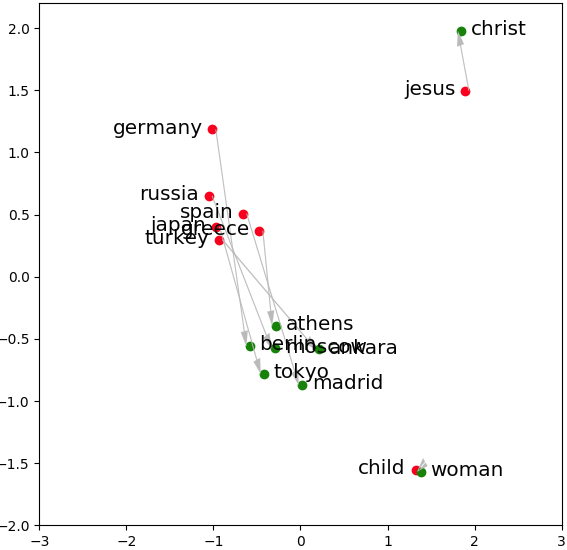
\includegraphics[width=3in,height=3in]{files/2.png}}
	\subfloat[Basic skip gram model]{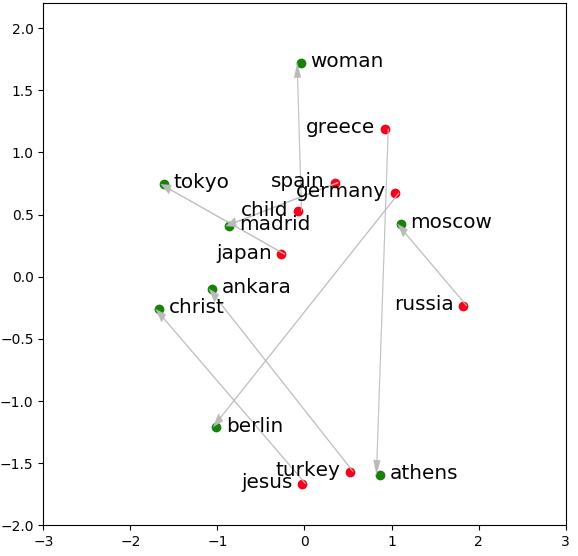
\includegraphics[width=3in,height=3in]{files/1.png}}
	\caption{Two-dimensional PCA projection of the \textbf{300-dimensional} skip gram vectors of countries and their capital cities trained on \textbf{English language} in 100,000 iterations on subset of dataset \texttt{Text8}. Countries(Red labels)and Captials(green labels)}\label{fig:t}
\end{figure}
\begin{figure}[htbp]
	\centering
	\subfloat[KPCA skip gram model]{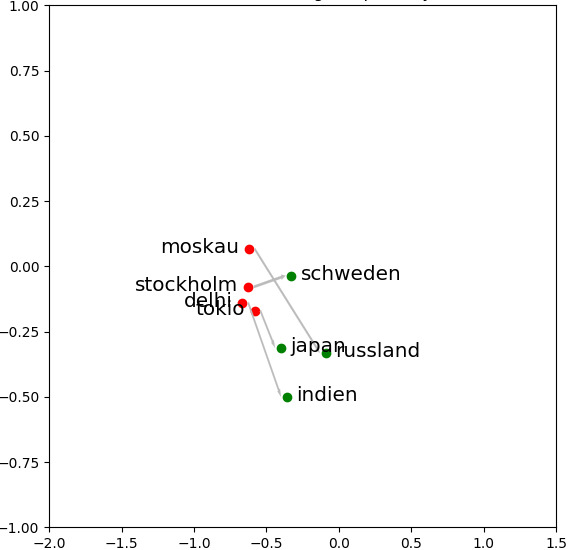
\includegraphics[width=3in,height=3in]{files/de1.png}}
	\subfloat[Basic skip gram model]{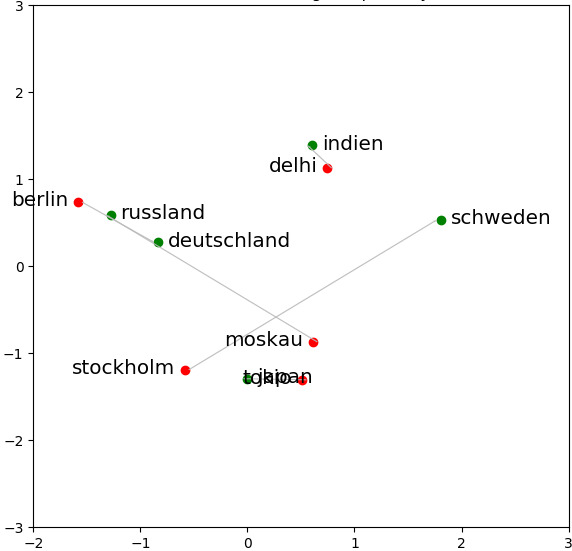
\includegraphics[width=3in,height=3in]{files/de2.png}}
	\caption{Two-dimensional PCA projection of the \textbf{300-dimensional} Skip-gram vectors of countries and their capital cities trained on \textbf{German language} in 100,000 iterations on subset of dataset \texttt{news.2013.de.shuffled.corpus}. Countries(Red labels)and Captials(green labels)}\label{fig:d}
\end{figure}

We have also calculated the accuracy of word analogy task using a \texttt{comprehensive test set}, which has been proposed and used by \cite{mikolov2013efficient} to evaluate their embeddings. The test consists of "semantic" and "syntactic" similarity questions. There are in total $19544$ questions which include relationships like: 
\begin{enumerate}
	\item adjective-to-adverb relationship
	\item capital-world relationship
	\item currency relationship
	\item plural-verbs relationship
	\item city-in-state relationship
	\item comparative relationship
	\item superlative relationship
	\item and many more...
\end{enumerate}
The test set computes the overall accuracy for all question types and is considered correctly answered only if the closest word to the vector computed is exactly the same as the correct word. Thus synonyms are considered as a wrong answer. \cite{mikolov2013efficient} has stated that to get these similarities, we need to train our model on a very large dataset. They have also reported that when they trained their model on a data set of size as big as \texttt{1.6 Billion or 768 Million words}, they obtained state of art accuracy even for \textbf{1 Epoch}.\\

In order to use this evaluation and to compare our model's results with basic skip gram as well as to the state-of-art results, we have trained our KPCA skip gram model and the basic skip gram model, on a smaller data set \textbf{Text8} as well on a huge data set, \textbf{en Wiki 2016}. We have also varied the number of epochs for training the smaller dataset(17 Million words) but only 1 epoch for larger dataset(1 Billion words) as stated by \cite{mikolov2013efficient}. Tests for the accuracies with different dictionary sizes for both the models have also been run.  
The performance of KPCA Skip gram and Basic Skip gram are reported in the tables \ref{ses1}, \ref{ses2} and \ref{tab:sesx}.  
\begin{table}[H]
	\hskip-1.0cm
	\begin{tabular}[htbp]{|l|l|l|l|l|}	
		\hline		
		\multicolumn{5}{|c|}{\textbf{KPCA Skip gram Embeddings vs Skip gram embeddings}} \\
	\hline
	Vocab Size&Model&Total Accuracy&Semantic Accuracy&Syntactic Accuracy\\ 
	\hline
	\multirow{2}{*}{Text8,V=20,000}
	&Basic Skip gram&0.08\%&0.00\%&0.13\%\\
	&KPCA Skip gram&9.35\%&2.27\%&13.40\%\\
	\hline
	\multirow{2}{*}{Text8,V=118,000}
	&Basic Skip gram&0.05\%&0.00\%&0.08\%\\
	&KPCA Skip gram&7.90\%&1.95\%&11.28\%\\
	\hline
\end{tabular}
\caption{Comparison of Word Analogy accuracy of the two models trained for \textbf{1 Epoch} using same parameters with 300-dimensional word vectors. NOTE: For vocabulary size of 118,000 for KPCA embeddings, we compute the KPCA for 20,000 words and the additional words(\textbf{OOV}) vectors are computed as discussed in \ref{oov}.}\label{ses1}
\end{table} 
From the accuracy values, shown in table, \ref{ses1}, it is very intuitive to see that our model performs very well when trained on a small data sets for which the basic skip gram model performs very badly. On further analysis of our model, we saw that the accuracy for semantic similarities are not so high. This can be attributed to the fact learning better semantic similarities is dependent on the skip gram model. Also the high accuracy of syntactic similarity of our model is attributed to the KPCA embeddings.\\
One question that arises is can basic skip gram model be trained on a relatively smaller dataset. The answer is "yes", but with the condition that the model should be trained for a number if epochs. This answer is backed by the results in table, \ref{ses2}. From the accuracies values of both the models in each epoch, we analyze that during the $1^{st}$ epoch, basic skip gram does not perform well but from the $2^{nd}$ epoch, it's performance accuracies caught up with our model, although there still remains some difference in the accuracies of the two models. Hence, considering accuracies from the $1^{st}$ epoch, we can easily say that training of our model is faster than the basic skip gram. 
\begin{table}[H]
	\centering
	\renewcommand{\arraystretch}{1.2}
	\begin{tabular}{|p{3cm}|c|c|c|c|c|c|c|}
		\hline
		\multirow{2}{5cm}{\textbf{No.of EPOCHS}} & \multicolumn{3}{c|}{\textbf{Skip-gram Model accuracy}} & \multicolumn{3}{c|}{\textbf{KPCA Skip-gram Model accuracy}}\\
		% \hline
		% \textbf{Inactive Modes} & \textbf{Description}\\
		\cline{2-7}
		& \textbf{Total} & \textbf{Semantic} & \textbf{Syntactic} & \textbf{Total} & \textbf{Semantic} & \textbf{Syntactic}\\
		%\hhline{~--}
		\hline
		1st Epoch&0.08\%&0.0\%&0.13\%&9.35\%&2.27\%&13.40\%\\ \hline
		2nd Epoch&7.15\%&2.12\%&9.56\%&8.77\%&2.92\%&12.57\%\\ \hline
		3rd Epoch&9.94\%&2.70\%&14.07\%&10.23\%&3.10\%&14.53\%\\ \hline
	\end{tabular}
	\caption{Word Analogy accuracy of both models through different epochs on Semantic-Syntactic data set}\label{ses2}
\end{table}
Finally, we would also like to compare accuracies achieved by our model to the basic skip grams' accuracies, when trained on a huge data set for 1 epoch. Therefore, we also evaluated our model against the skip gram model, trained on a very large dataset,  \texttt{English wikipedia 2016 dump}. This data set is very large, having 1 Billion words. Due to computation limitations, we trained the skip gram and KPCA skip gram using the vocabulary size of 30,000 words.
As we have discussed earlier that our model has an advantage of having embedded morphological similarity in the input vector, therefore if trained with numerous example, our model intuitively should perform better than the skip gram model. This intuition is backed by the accuracies result from the table, in table, \ref{tab:sesx}. The main point to notice in the table, \ref{tab:sesx}, is the difference in accuracies of syntactic similarities of both the models. This can again be attributed to the fact that morphological similarity are more related to the syntactic similarity.\\
In summary, after evaluating our model against the skip gram model using the evaluation techniques, we can say the KPCA skip gram model performs bette than the basic skip gram model. We can also say that our model has even better performance on syntactic similarity or on smaller datasets.

 \begin{table}[H]
 	\hskip-1.5cm
 	\begin{tabular}[htbp]{|l|l|l|l|l|}	
 		\hline		
 		\multicolumn{5}{|c|}{\textbf{KPCA Skip gram Model vs Skip gram Model On wiki2016}} \\
 		\hline
 		Vocab Size&Model&Total Accuracy&Semantic Accuracy&Syntactic Accuracy\\ 
 		\hline
 		\multirow{2}{*}{Skipgram model}
 		&Uptil 10,000 steps&0.05\%&0.00\%&0.11\%\\
 		&Full epoch&46.31\%&54.26\%&39.74\%\\
 		\hline
 		\multirow{2}{*}{KPCA skip gram model}
 		&Uptil 10,000 steps&4.52\%&4.47\%&4.56\%\\
 		&Full epoch&58.01\%&57.91\%&58.09\%\\
 		\hline
 	\end{tabular}
 	\caption{Comparison of architectures of the two models trained for \textbf{1 Epoch} using same parameters with 300-dimensional word vectors on \textbf{enWikidump} of size 1 Billion words with Vocabulary size 30,000}\label{tab:sesx}
 \end{table}
 The results in the table, \ref{tab:sesx}, shows that our model learns the subtle relations between words very quickly, as we can see that the accuracy of our model is higher than the skip gram model even in 100,000 steps of 1 epoch. Even after completing the whole epoch, our model performs better in terms of accuracy. This can again be attributed to the fact that if vectors are initialized with morphological similarity then we don't need to show a large number of examples to the model to learn the relationships.
	\chapter{Conclusion and Future Work}
\label{cha:concl}

\section{Improvement To the Skip Gram Model}

In this thesis work, we have explored the importance of morphological similarities in generating word embeddings. We took a step by step approach from defining a similarity function between words to generating the kernelized PCA embeddings to feeding the skip gram model with these KPCA embeddings. We also evaluated at each step, how each algorithm performed and which parameters are best suited. The main goal of this work was to explore, the idea of enriching the word embeddings, generated by skip gram model, with the morphological information. This morphological information is encoded in the KPCA embeddings which are obtained by applying KPCA on some defined similarity function of the words. Therefore when we initialized the skip gram model by these morphological similarity words, we found that our model achieve fairly good accuracies in fewer iterations. We have also evaluated the embeddings by intrinsic methods of "word similarity" and "word analogy". In every task, our model has performed better than the basic skip gram model. From the evaluation results, we understood that, a skip gram model can learn similarity between words based on context only when it has seen sufficient number of examples. This can be achieved by either training the skip gram model with a huge dataset or training it with a relatively smaller dataset but with numerous epochs. 
But when we fed the skip gram model with morphological embeddings, it already has a good initial point from where it can improve these embeddings. This works, especially well, when we are training on a morphologically rich language since semantic and morphological similarities converges in these languages therefore feeding the network with KPCA embeddings, gives a boost to the network enabling it to learn meaningful word vectors even faster than the non morphological languages.\\
We also observed that it is possible to obtain fair quality word vectors using KPCA skip gram model in just 1 epoch after training even on a smaller data set. Since skip gram model does not perform well when trained on a relatively smaller data set, our approach can be used in situations where we don't have a huge data set. One such case arises when we have a very new data set such as NEWS articles. Because the current news events changes every often, it is difficult to get good word embeddings for new words which get associated with some context. For example: When Donald Trump won the presidential elections, the newly trained word embeddings for the word 'president' were still lie closer to 'obama' and not close to 'trump'. This is because the skip gram model has not seen enough examples where word 'president' is used in context of 'trump'. In such situations, our approach can do better as we can train on smaller datasets. \\


\section{Improving KPCA Skip Gram Model}
While the KPCA skip gram model, gave good results, there still exists a lot of scope for the improvements which are enumerated as follows:
\begin{itemize}
	\item Selecting number of grams to be considered for generating \textit{n}-gram.
	\begin{itemize}
		\item In this work, we have selected the value of \textit{n} to be 3 and 4 for English and German language for generating \textit{n}-grams. This is an important hyperparmeter which determines the quality of the KPCA embeddings. In this work, we hard coded this parameter but this need to be generalized as n=3, might not give good quality n-grams(morphemes) for some language. This can be generalized by generating different set of similarity measures using different values of \texttt{n = 2,3,4,5,..} and then averaging the similarity for the two words for these set. Thus we can have a generalized model for getting similarity between the words.  
	\end{itemize}
	\item Iterative Kernel PCA for a very large vocabulary
	\begin{itemize}
		\item Since Kernel PCA for matrices of very large dimensions are very computationally expensive, there have been some research going on how to do this iteratively. This is an open research topic that can be explored in future. There are "gain adaptation methods" that improve convergence of the kernel Hebbian algorithm (KHA) for iterative kernel PCA. These methods have demonstrated the scalability by performing kernel PCA on the MNIST database.
	\end{itemize} 
	\item Exploring KPCA fastText
		\begin{itemize}
		\item Although we can obtain the KPCA vector of an out-of-vocabulary word using KPCA projection matrix, but these vector are only enriched with the morphological similarities. We still miss the vector representations encoded with semantic and syntactic similarities. This can be achieved using fastText approach. If we can adapt our KPCA skip gram model according to the fastText, then we can also generate out-of-vocabulary words which are enriched in semantic, syntactic and morphological similarities.  
	\end{itemize} 
\end{itemize}

	%\begin{appendix}
	%	\input{appendix}
	%\end{appendix}
	
	%references
	\bibliographystyle{apalike}
\bibliography{refs}

	
\end{document}